\special{! TeXDict begin /landplus90{true}store end }

\documentclass[xga]{xdvislides}
\usepackage[landscape]{geometry}
\usepackage{graphics}
\usepackage{graphicx}
\usepackage{colordvi}
\usepackage{multirow}
\usepackage[normalem]{ulem}

\usepackage{fancyvrb}
\fvset{fontfamily=courier,commandchars=\\\{\}}

\begin{document}
\setfontphv

%%% Headers and footers
\lhead{\slidetitle}                               % default:\lhead{\slidetitle}
\chead{CS615 - Aspects of System Administration}% default:\chead{\relax}
\rhead{Slide \thepage}                       % default:\rhead{\sectiontitle}
\lfoot{\Gray{HTTPS, TLS, SMTP}}% default:\lfoot{\slideauthor}
\cfoot{\relax}                               % default:\cfoot{\relax}
\rfoot{\Gray{\today}}

\newcommand{\smallish}{\fontsize{16}{16}\selectfont}

\vspace*{\fill}
\begin{center}
	\Hugesize
		CS615 - Aspects of System Administration\\ [1em]
		HTTPS, TLS, SMTP\\ [1em]
	\hspace*{5mm}\blueline\\ [1em]
	\Normalsize
		Department of Computer Science\\
		Stevens Institute of Technology\\
		Jan Schaumann\\
		\verb+jschauma@stevens.edu+\\
		\verb+https://stevens.netmeister.org/615/+
\end{center}
\vspace*{\fill}


\subsection{HTTP}
\begin{center}
	\includegraphics[scale=0.3]{pics/stevens-ec2.eps} \\
	\verb+http://ec2-54-160-173-145.compute-1.amazonaws.com/+
\end{center}

\subsection{HTTP}
\begin{verbatim}
$ sudo tcpdump -w post.pcap port 80 2>/dev/null &
$ fg
^C
$ sudo chmod a+r post.pcap
\end{verbatim}

Now use {\tt tcpdump(1)} to extract the plain text data you sent
to the web server from your {\tt pcap} file.


\subsection{HTTP}
\small
\begin{verbatim}
14:14:35.348492 IP 172.16.1.20.52941 > 54.160.173.145.80: Flags [P.], seq 1:668,
        0x0000:  4500 02cf 0000 4000 4006 a6d3 ac10 0114  E.....@.@.......
        0x0010:  36a0 ad91 cecd 0050 6d61 ffbe ab1f 5284  6......Pma....R.
        0x0020:  8018 080a 8dc1 0000 0101 080a 53ec 8097  ............S...
        0x0030:  0000 0001 504f 5354 202f 6367 692d 6269  ....POST./cgi-bi
        0x0040:  6e2f 706f 7374 2e63 6769 2048 5454 502f  n/post.cgi.HTTP/
        0x0050:  312e 310d 0a48 6f73 743a 2065 6332 2d35  1.1..Host:.ec2-5
        0x0060:  342d 3136 302d 3137 332d 3134 352e 636f  4-160-173-145.co
        0x0070:  6d70 7574 652d 312e 616d 617a 6f6e 6177  mpute-1.amazonaw
        0x0080:  732e 636f 6d0d 0a43 6f6e 6e65 6374 696f  s.com..Connectio
        0x0090:  6e3a 206b 6565 702d 616c 6976 650d 0a43  n:.keep-alive..C
        0x00a0:  6f6e 7465 6e74 2d4c 656e 6774 683a 2037  ontent-Length:.7
        0x00b0:  310d 0a43 6163 6865 2d43 6f6e 7472 6f6c  1..Cache-Control
        0x00c0:  3a20 6d61 782d 6167 653d 300d 0a4f 7269  :.max-age=0..Ori
        0x00d0:  6769 6e3a 2068 7474 703a 2f2f 6563 322d  gin:.http://ec2-
        0x00e0:  3534 2d31 3630 2d31 3733 2d31 3435 2e63  54-160-173-145.c
        0x00f0:  6f6d 7075 7465 2d31 2e61 6d61 7a6f 6e61  ompute-1.amazona
        0x0100:  7773 2e63 6f6d 0d0a 5570 6772 6164 652d  ws.com..Upgrade-
        0x0110:  496e 7365 6375 7265 2d52 6571 7565 7374  Insecure-Request
        0x0120:  733a 2031 0d0a 444e 543a 2031 0d0a 436f  s:.1..DNT:.1..Co
[...]
        0x0250:  6469 6e67 3a20 677a 6970 2c20 6465 666c  ding:.gzip,.defl
        0x0260:  6174 650d 0a41 6363 6570 742d 4c61 6e67  ate..Accept-Lang
        0x0270:  7561 6765 3a20 656e 2d55 532c 656e 3b71  uage:.en-US,en;q
        0x0280:  3d30 2e39 0d0a 0d0a 6a5f 7573 6572 6e61  =0.9....j_userna
        0x0290:  6d65 3d6a 7363 6861 756d 6126 6a5f 7061  me=jschauma&j_pa
        0x02a0:  7373 776f 7264 3d6e 6f74 2b72 6561 6c6c  ssword=not+reall
        0x02b0:  792b 6d79 2b70 6173 7377 6f72 6426 5f65  y+my+password&_e
        0x02c0:  7665 6e74 4964 5f70 726f 6365 6564 3d ventId_proceed=

\end{verbatim}
\Normalsize

\subsection{HTTPS}
\begin{verbatim}
$ </dev/null openssl s_client -connect ec2-54-160-173-145.compute-1.amazonaws.com:443 |
        openssl x509 -text -noout | more
$ sudo tcpdump -w post.pcap port 443 2>/dev/null &
$ fg
^C
$ sudo chmod a+r post.pcap
\end{verbatim}
\small
\begin{verbatim}
14:24:13.686601 IP 104.244.42.130.443 > 172.16.1.20.51827: Flags [P.], seq 1:73, ack 242, win
1701, options [nop,nop,TS val 418195978 ecr 1408582944], length 72
        0x0000:  4500 007c a9f2 4000 3106 5eef 68f4 2a82  E..|..@.1.^.h.*.
        0x0010:  ac10 0114 01bb ca73 b729 f478 4c0f efbd  .......s.).xL...
        0x0020:  8018 06a5 dce5 0000 0101 080a 18ed 2a0a  ..............*.
        0x0030:  53f5 4520 1703 0300 4394 0c3d 7475 a12d  S.E.....C..=tu.-
        0x0040:  0213 03b6 7cfa d081 27af d0a6 fdcd a5a5  ....|...'.......
        0x0050:  7a40 c070 6548 43fb 4264 1602 29ce 45aa  z@.peHC.Bd..).E.
        0x0060:  9705 0b7b ba7b e169 4753 5e3e 8741 c3d1  ...{.{.iGS^>.A..
        0x0070:  aec5 15c1 a3f9 b583 c07a 9ab8            .........z..
14:24:13.686643 IP 172.16.1.20.51827 > 104.244.42.130.443: Flags [.], ack 73, win 2046,
options [nop,nop,TS val 1408582975 ecr 418195978], length 0
        0x0000:  4500 0034 0000 4000 4006 fa29 ac10 0114  E..4..@.@..)....
        0x0010:  68f4 2a82 ca73 01bb 4c0f efbd b729 f4c0  h.*..s..L....)..
        0x0020:  8010 07fe 9e12 0000 0101 080a 53f5 453f  ............S.E?
        0x0030:  18ed 2a0a
\end{verbatim}
\Normalsize

\subsection{HTTPS}
HTTPS stands for... \\

HTTP over SSL.

\subsection{HTTPS}
HTTPS stands for... \\

\sout{HTTP over SSL.} \\

HTTP over TLS.

\subsection{HTTPS}
HTTPS stands for... \\

\sout{HTTP over SSL.} \\

\sout{HTTP over TLS.} \\

Secure HTTP.

\subsection{HTTPS}
HTTPS stands for... \\

\sout{HTTP over SSL.} \\

\sout{HTTP over TLS.} \\

\sout{Secure HTTP.} \\

HTTP Secure.

\subsection{HTTPS}
HTTPS stands for... \\

\sout{HTTP over SSL.} \\

\sout{HTTP over TLS.} \\

\sout{Secure HTTP.} \\

HTTP Secure. \\

But it uses TLS.  And used to use SSL. Although
hopfully not any more.  Although probably still. \\

SSL is dead.  Don't use it.  Seriously, don't. \\

We should really only call it TLS.  HTTPT.

\subsection{TLS}
\begin{center}
	\includegraphics[scale=0.7]{pics/OSI_Model.eps}
\end{center}

\subsection{TLS}
Transport Layer Security
\begin{itemize}
	\item set of cryptographic protocols
	\item operates on layer 6 of OSI stack (Presentation Layer) (or 5? 4? 7? none? all?)
	\item independent of HTTP
	\item TLS 1.2 (RFC5246) standardized in 2008
	\item TLS 1.3 (RFC8446) standardized in 2018
\end{itemize}
\addvspace{.5in}
Two distinct security mechanisms:
\begin{enumerate}
	\item encryption of data in transit
	\item authentication of parties
\end{enumerate}

\subsection{TLS}
Protocol:
\begin{itemize}
	\item Client Hello, present list of supported cipher suites
	\item Server Hello, chosen cipher suite
	\item Server Certificate
	\item (Server Key Exchange Message), (Client Certificate Request), (Client Certificate)
	\item Client Key Exchange Message
	\item (Certificate Verify)
	\item (Client Change Cipher Spec), (Server Change Cipher Spec)
\end{itemize}
\vspace{.5in}
See also: \verb+https://tls.ulfheim.net/+

\subsection{TLS}
\begin{center}
	\includegraphics[scale=0.4]{pics/wireshark.eps}
\end{center}

\subsection{TLS}
\begin{verbatim}
$ openssl s_client -connect www.stevens.edu:443
[...]
New, TLSv1.2, Cipher is ECDHE-RSA-CHACHA20-POLY1305
Server public key is 2048 bit
Secure Renegotiation IS supported
SSL-Session:
    Protocol  : TLSv1.2
    Cipher    : ECDHE-RSA-CHACHA20-POLY1305
    Session-ID: 32FB0E95CA87601D671ACF26AD3B7BF9C288C8CCF1C1FF8116018E7DC8890448
    Session-ID-ctx: 
    Master-Key: A7B50CCD8F08745B019163C107BCBB52DFB67453BAF90E09F48B0E393E7E05401F1754E67E0C6005F656A55B493444CA
    PSK identity: None
    PSK identity hint: None
    SRP username: None
    TLS session ticket lifetime hint: 64800 (seconds)
    TLS session ticket:
\end{verbatim}

\subsection{TLS}
\smallish
\begin{verbatim}
$ openssl s_client -connect www.stevens.edu:443 | \
        openssl x509 -text -noout
[...]
        Serial Number:
            9a:9e:f8:47:2d:aa:4b:a3:e6:be:85:b7:9d:51:18:d6
    Signature Algorithm: sha256WithRSAEncryption
        Issuer: C=US, ST=MI, L=Ann Arbor, O=Internet2, OU=InCommon, CN=InCommon RSA Server CA
        Validity
            Not Before: Dec  4 00:00:00 2018 GMT
            Not After : Dec  4 23:59:59 2019 GMT
        Subject: C=US/postalCode=07030, ST=NJ,
                 L=Hoboken/street=Castle Point on Hudson,
                 O=Stevens Institute of Technology, OU=IT,
                 CN=*.stevens.edu
[...]
            X509v3 Subject Alternative Name: 
                DNS:*.stevens.edu, DNS:stevens.edu
\end{verbatim}
\Normalsize
Note the absence of 'stevens-tech.edu' names...

% \subsection{TLS}
% Setting up a Man in the Middle attack site: \\
% 
% 1. start instance \\
% 
% 2. {\tt openssl req -x509 -nodes -days 30 -sha256 \
%         -newkey rsa:4096 -keyout mycert.pem -out mycert.pem}
% 
% 3. {\tt sudo openssl s\_server -WWW -accept 443 -cert mycert.pem} \\
% 
% 4. {\tt curl https://www.stevens.edu/sit/ > index.html} \\
% 
% 4. go to {\tt https://<instance>/} \\
 
\subsection{TLS Authentication}
Use of X.509:
\begin{itemize}
	\item public key certificates
	\item certificate revocation lists (CRLs) / Online Certificate Status Protocol (OCSP)
	\item certificate path validation under a Public Key Infrastructure (PKI)
	\item certificate chains depend on trust anchors
\end{itemize}

\subsection{TLS}
1. User / Company generates a {\em Certificate Signing Request} (CSR),
containing:

\begin{itemize}
	\item identifying information (distinguished name etc.)
	\item signature of data by private key
	\item chosen public key
\end{itemize}

\subsection{TLS}
1. User / Company generates a {\em Certificate Signing Request} (CSR) \\

2. CSR submitted to Certificate Authority (CA) \\

\subsection{TLS}
1. User / Company generates a {\em Certificate Signing Request} (CSR) \\

2. CSR submitted to Certificate Authority (CA) \\

3. CA verifies information \\

\subsection{TLS}
1. User / Company generates a {\em Certificate Signing Request} (CSR) \\

2. CSR submitted to Certificate Authority (CA) \\

3. CA verifies information \\

4. CA returns certificate signed with its private key \\

\subsection{TLS}
1. User / Company generates a {\em Certificate Signing Request} (CSR) \\

2. CSR submitted to Certificate Authority (CA) \\

3. CA verifies information \\

4. CA returns certificate signed with its private key \\

5. clients can verify signatures against trusted {\em root CAs} \\

\subsection{TLS}
\begin{center}
	\includegraphics[scale=0.57]{pics/csr-process.eps}
\end{center}



\subsection{TLS Pitfalls}
\begin{center}
	\includegraphics[scale=0.6]{pics/roots.eps} \\
	195 root CAs on this laptop...
\end{center}

\subsection{TLS Pitfalls}
Just because a site has a valid certificate does not
mean it's a trustworthy site. \\

\begin{verbatim}
https://ec2-54-160-173-145.compute-1.amazonaws.com/

https://www.netmeister.org/tumblr/

https://www.netmeister.org/owa/auth/logon.aspx
\end{verbatim}


\subsection{TLS Pitfalls}
Lack of universal HTTPS exposes users to significant
risks; many sites don't understand the importance of
authentication and encryption for non-sensitive content. \\

\verb+https://is.gd/ghiOhU+ \\

Middle boxes, often advertized as a security
mechanism, are actively harmful to users and prohibit
secure protocol development. \\

In order to serve content, you need to have the
private key $ => $ privkey available at perimeter and
exposed, high-risk systems. \\

Rotation/renewal of keys requires routine processes,
which may further expose the private key. \\

Control of a CA or a CA's key grants you near
universal powers. \\


\subsection{TLS Pitfalls}
Complex protocols, buggy implementations, intentional
weaknesses and backwards compatibility are just the
high level points.

\begin{itemize}
	\item SSLv2 obsoleted in 1996; 2016: DROWN attack
	\item SSLv3 obsoleted in 1999; 2014: POODLE attack
	\item BEAST, CRIME, BREACH, HEARTBLEED, GotoFail...
	\item obsolete and broken algorithms widely used (RC4, MD5, SHA1, ...)
\end{itemize}

\subsection{TLS}
Additional related topics:
\begin{itemize}
	\item HSTS and TLS stripping attacks
	\item HPKP and Trust On First Use (TOFU)
	\item Certificate Transparency
	\item Content Security Policy (CSP)
	\item ``Secure'' cookies vs. HttpOnly cookies
	\item attacks on domain name registrars
\end{itemize}
\addvspace{.5in}
Security is difficult.  More on that in a future
lecture.


\newpage
\vspace*{\fill}
\begin{center}
    \Hugesize
        Hooray! \\ [1em]
    \hspace*{5mm}
    \blueline\\
    \hspace*{5mm}\\
        5 Minute Break
\end{center}
\vspace*{\fill}

\subsection{Email... still popular}
Bad news, everybody: Slack has not yet replaced email.

\subsection{Email... still popular}
Good news, everybody: Slack has not yet replaced email. (And it's not going to.)
\\

\begin{itemize}
	\item {\bf 4.6 billion} - number of email accounts.
	\item {\bf 269 billion} - Average number of email messages per day. \\
		That's 3.1 million emails {\em per second}.
	\item {\bf 121} - Average number of emails an office worker receives.
	\item {\bf 42} - Percentage of Americans that check their email in the bathroom.
	\item {\bf 18} - Percentage of Americans that check their email while driving.
	\item {\bf $>$70} - Percentage of emails that are Spam.
\end{itemize}

\subsection{The Mail System}
Divided into:
\begin{itemize}
	\item {\em Mail User Agent} or MUA, such as {\tt mutt(1)}, {\em Mail.app}, {\em Outlook}, a browser (ugh) ...
	\item {\em Mail Transfer Agent} or MTA, such as {\em postfix},
		{\em sendmail}, {\em qmail}, ...
	\item {\em Mail Delivery Agent} or MDA, such as {\em procmail}
	\item {\em Access Agent} providing access via {\em POP}, {\em IMAP} etc.
\end{itemize}
\vspace{.5in}
In addition, many MUAs nowadays interpret HTML:
\begin{itemize}
	\item browser now the most common MUA
	\item facilitates phishing (via link obscuring, logos etc.)
	\item facilitates tracking (via beacons, cookies)
\end{itemize}


\subsection{Sending...}
\begin{verbatim}
# tcpdump -i xennet0 -w /tmp/t.out port not 22 2>/dev/null &
# mail -s "CS615 - SMTP Exercise" jschauma@netmeister.org -f jschauma@stevens.edu
Hello,

SMTP is so simple!

-Jan
.
EOT
# fg
tcpdump -i xennet0 -w /tmp/t.out port not 22 2>/dev/null
^C
\end{verbatim}

\subsection{Sending...}
\begin{verbatim}
# tail -6 /var/log/maillog
Mar 25 14:19:59 ip-10-168-152-198 postfix/pickup[5939]: A76DB2FFC2:
        uid=0 from=<jschauma@stevens.edu>
Mar 25 14:19:59 ip-10-168-152-198 postfix/cleanup[5564]: A76DB2FFC2:
        message-id=<20190325141959.A76DB2FFC2@ip-10-168-152-198.ec2.internal>
Mar 25 14:19:59 ip-10-168-152-198 postfix/qmgr[1846]: A76DB2FFC2:
        from=<jschauma@stevens.edu>, size=386, nrcpt=1 (queue active)
Mar 25 14:19:59 ip-10-168-152-198 postfix/smtp[7163]: connect to
        panix.netmeister.org[2001:470:30:84:e276:63ff:fe72:3900]:25:
        No route to host
Mar 25 14:20:00 ip-10-168-152-198 postfix/smtp[7163]: A76DB2FFC2:
        to=<jschauma@netmeister.org>, relay=panix.netmeister.org[166.84.7.99]:25,
        delay=0.48, delays=0.03/0.01/0.29/0.15, dsn=2.0.0,
        status=sent (250 2.0.0 Ok: queued as 2223965341)
Mar 25 14:20:00 ip-10-168-152-198 postfix/qmgr[1846]: A76DB2FFC2: removed
\end{verbatim}

\subsection{Sending...}
\begin{verbatim}
# tcpdump -n -t -t smtp-client.pcap port 53
IP 10.168.152.198.63685 > 172.16.0.23.53: 1736+ MX? netmeister.org. (32)
IP 172.16.0.23.53 > 10.168.152.198.63685: 1736 1/0/0 MX panix.netmeister.org. 50 (54)
IP 10.168.152.198.63684 > 172.16.0.23.53: 64083+ A? panix.netmeister.org. (38)
IP 172.16.0.23.53 > 10.168.152.198.63684: 64083 1/0/0 A 166.84.7.99 (54)
IP 10.168.152.198.63683 > 172.16.0.23.53: 16542+ AAAA? panix.netmeister.org. (38)
IP 172.16.0.23.53 > 10.168.152.198.63683: 16542 1/0/0 AAAA 2001:470:30:84:e276:63ff:fe72:3900 (66)
\end{verbatim}
\vspace{.5in}
\begin{verbatim}
$ host -t mx netmeister.org
netmeister.org mail is handled by 50 panix.netmeister.org.
$ host panix.netmeister.org
panix.netmeister.org has address 166.84.7.99
panix.netmeister.org has IPv6 address 2001:470:30:84:e276:63ff:fe72:3900
$ 
\end{verbatim}

\subsection{Sending...}
\begin{verbatim}
$ tcpdump -n -t -r smtp-client.pcap 'tcp[tcpflags] & tcp-push != 0 and port 25'
IP 166.84.7.99.25 > 10.168.152.198.65528: Flags [P.], seq 1:41, ack 1
        SMTP: 220 panix.netmeister.org ESMTP Postfix
IP 10.168.152.198.65528 > 166.84.7.99.25: Flags [P.], seq 1:38, ack 41
        SMTP: EHLO ip-10-168-152-198.ec2.internal
IP 166.84.7.99.25 > 10.168.152.198.65528: Flags [P.], seq 41:174, ack 38
        SMTP: 250-panix.netmeister.org
IP 10.168.152.198.65528 > 166.84.7.99.25: Flags [P.], seq 38:159, ack 174
        SMTP: MAIL FROM:<jschauma@stevens.edu> SIZE=386
IP 166.84.7.99.25 > 10.168.152.198.65528: Flags [P.], seq 174:239, ack 159
        SMTP: 250 2.1.0 Ok
IP 10.168.152.198.65528 > 166.84.7.99.25: Flags [P.], seq 159:554, ack 239
        SMTP: Received: by ip-10-168-152-198.ec2.internal (Postfix, from userid 0)
IP 166.84.7.99.25 > 10.168.152.198.65528: Flags [P.], seq 239:290, ack 554
        SMTP: 250 2.0.0 Ok: queued as 2223965341
\end{verbatim}

\subsection{SMTP Codes}
SMTP codes consist of three digits in five classes:
\begin{itemize}
	\item {\bf 1xx} --  Mail server has accepted the command, but does not yet
		take any action. A confirmation message is required.
	\item {\bf 2xx} --  Mail server has completed the task successfully
		without errors.
	\item {\bf 3xx} --  Mail server has understood the request, but requires
		further information to complete it.
	\item {\bf 4xx} --  Mail server has encountered a temporary failure. If
		the command is repeated without any change, it might be
		completed. Try again, it may help!
	\item {\bf 5xx} --  Mail server has encountered a fatal error. Your
		request can't be processed.
\end{itemize}


\subsection{Sending...}
\begin{Verbatim}
$ telnet panix.netmeister.org 25
Trying 2001:470:30:84:e276:63ff:fe72:3900...
telnet: connect to address 2001:470:30:84:e276:63ff:fe72:3900: No route to host
Trying 166.84.7.99...
Connected to panix.netmeister.org.
Escape character is '^]'.
220 panix.netmeister.org ESMTP Postfix
\textbf{EHLO ip-10-168-152-198.ec2.internal}
250-panix.netmeister.org
[...]
\textbf{MAIL FROM: <jschauma@stevens.edu>}
250 2.1.0 Sender OK
\textbf{RCPT TO: <jschauma@netmeister.org>}
250 2.1.5 Recipient OK
\end{Verbatim}

\subsection{Sending...}
\begin{Verbatim}
\textbf{DATA}
354 Start mail input; end with <CRLF>.<CRLF>
\textbf{To: jschauma@netmeister.org}
\textbf{Subject: CS615 - SMTP Exercise}
\textbf{Mon, 25 Mar 2019 14:19:59 +0000 (UTC)}
\textbf{From: Charlie Root <jschauma@stevens.edu>}

\textbf{Hello,}

\textbf{SMTP is so simple!}

\textbf{-Jan}
\textbf{.}
250 2.0.0 Ok: queued as 522DF65341
\end{Verbatim}

\subsection{Sending...}
\begin{center}
	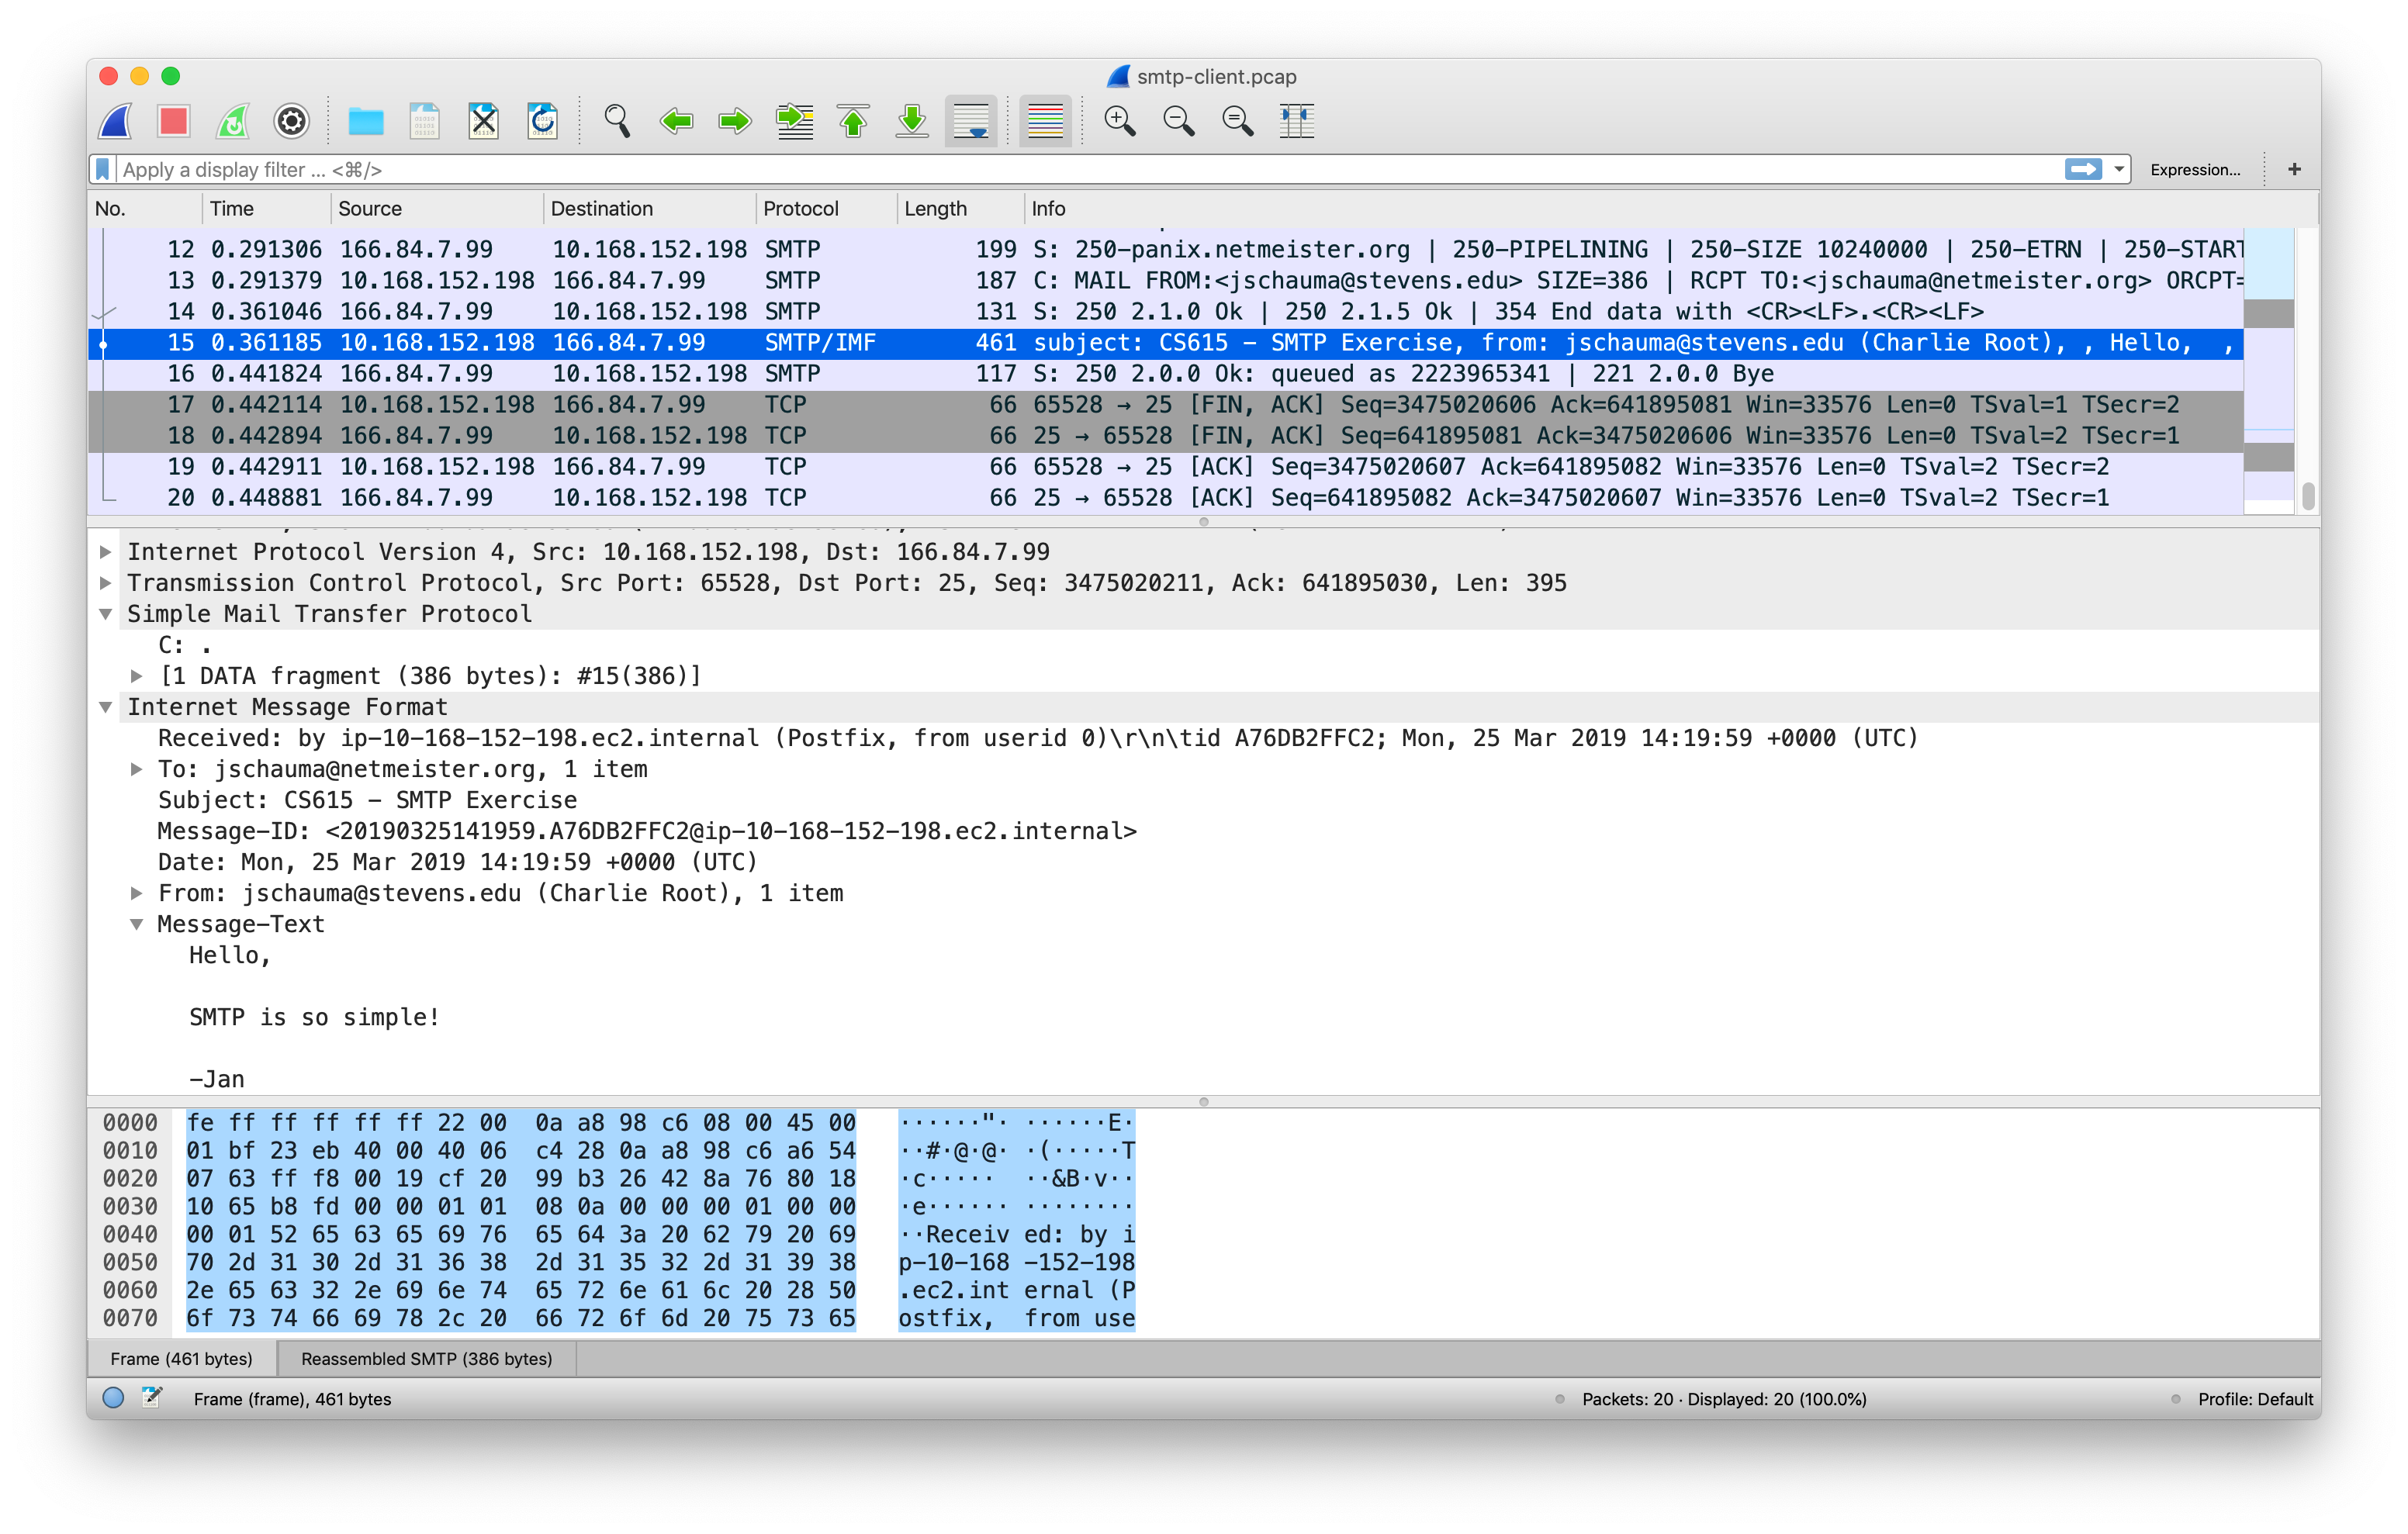
\includegraphics[scale=0.35]{pics/wireshark-smtp.eps}
\end{center}

\subsection{Receiving...}
\begin{verbatim}
$ tcpdump -n -t -r smtp-server.pcap 'tcp[tcpflags] & tcp-push != 0 and port 25'
IP 166.84.7.99.25 > 54.160.173.145.65528: Flags [P.], seq 641894792:641894832, ack 3475020053
        SMTP: 220 panix.netmeister.org ESMTP Postfix
IP 54.160.173.145.65528 > 166.84.7.99.25: Flags [P.], seq 1:38, ack 40
        SMTP: EHLO ip-10-168-152-198.ec2.internal
IP 166.84.7.99.25 > 54.160.173.145.65528: Flags [P.], seq 40:173, ack 38
        SMTP: 250-panix.netmeister.org
IP 54.160.173.145.65528 > 166.84.7.99.25: Flags [P.], seq 38:159, ack 173
        SMTP: MAIL FROM:<jschauma@stevens.edu> SIZE=386
IP 166.84.7.99.25 > 54.160.173.145.65528: Flags [P.], seq 173:238, ack 159
        SMTP: 250 2.1.0 Ok
IP 54.160.173.145.65528 > 166.84.7.99.25: Flags [P.], seq 159:554, ack 238
        SMTP: Received: by ip-10-168-152-198.ec2.internal (Postfix, from userid 0)
IP 166.84.7.99.25 > 54.160.173.145.65528: Flags [P.], seq 238:289, ack 554
        SMTP: 250 2.0.0 Ok: queued as 2223965341
\end{verbatim}

\subsection{Receiving}
\begin{verbatim}
$ sudo grep 2223965341 /var/log/maillog
<mail.info>Mar 25 10:20:01 panix postfix/smtpd[5089]: 2223965341:
        client=ec2-54-160-173-145.compute-1.amazonaws.com[54.160.173.145]
<mail.info>Mar 25 10:20:01 panix postfix/cleanup[10085]: 2223965341:
        message-id=<20190325141959.A76DB2FFC2@ip-10-168-152-198.ec2.internal>
<mail.info>Mar 25 10:20:01 panix postfix/qmgr[1932]: 2223965341:
        from=<jschauma@stevens.edu>, size=627, nrcpt=1 (queue active)
<mail.info>Mar 25 10:20:21 panix postfix/pipe[10375]: 2223965341:
        to=<jschauma@netmeister.org>, relay=spamassassin, delay=20, delays=0.15/0/0/20,
        dsn=2.0.0, status=sent (delivered via spamassassin service)
<mail.info>Mar 25 10:20:21 panix postfix/qmgr[1932]: 2223965341: removed
\end{verbatim}

\subsection{Receiving}
\begin{center}
	\includegraphics[scale=0.35]{pics/wireshark-smtp-server.eps}
\end{center}

%% XXX
%\subsection{Sending...}
%\begin{verbatim}
%# tcpdump -i xennet0 -w /tmp/t.out port not 22 2>/dev/null &
%# mail -s "CS615 - SMTP Exercise" jschauma@stevens.edu -f jschauma@stevens.edu
%Hello,
%
%SMTP is so simple!
%
%-Jan
%.
%EOT
%# fg
%tcpdump -i xennet0 -w /tmp/t.out port not 22 2>/dev/null
%^C
%\end{verbatim}
%
%
%\subsection{Sending...}
%\begin{verbatim}
%# tail -5 /var/log/maillog
%Mar 17 19:07:46 ip-10-225-79-205 postfix/pickup[1937]:
%        981302FFB4: uid=0 from=<jschauma@stevens.edu>
%Mar 17 19:07:46 ip-10-225-79-205 postfix/cleanup[2252]:
%        981302FFB4: message-id=<20180317190746.981302FFB4@ip-10-225-79-205.ec2.internal>
%Mar 17 19:07:46 ip-10-225-79-205 postfix/qmgr[1662]:
%        981302FFB4: from=<jschauma@stevens.edu>, size=381, nrcpt=1 (queue active)
%Mar 17 19:07:47 ip-10-225-79-205 postfix/smtp[2285]:
%        981302FFB4: to=<jschauma@stevens.edu>, relay=spamfilter01.stevens.edu[155.246.14.37]:25,
%        delay=0.42, delays=0.02/0/0.17/0.23, dsn=2.0.0, status=sent (250 Ok: queued as 17A35227E1D4)
%Mar 17 19:07:47 ip-10-225-79-205 postfix/qmgr[1662]:
%        981302FFB4: removed
%\end{verbatim}
%
%\subsection{Sending...}
%\begin{verbatim}
%$ tcpdump -t -r /tmp/stevens-client.pcap port 53
%reading from PCAP-NG file /tmp/stevens-client.pcap
%IP 10.183.182.79.65506 > 172.16.0.23.domain: 43895+ MX? stevens.edu. (29)
%IP 172.16.0.23.domain > 10.183.182.79.65506: 43895 1/0/0 
%        MX stevens-edu.mail.protection.outlook.com. 0 (84)
%IP 10.183.182.79.65505 > 172.16.0.23.domain: 2757+ A?
%        stevens-edu.mail.protection.outlook.com. (57)
%IP 172.16.0.23.domain > 10.183.182.79.65505: 2757 2/0/0 A
%        104.47.37.36, A 104.47.36.36 (89)
%IP 10.183.182.79.65504 > 172.16.0.23.domain: 8847+ AAAA?
%        stevens-edu.mail.protection.outlook.com. (57)
%IP 172.16.0.23.domain > 10.183.182.79.65504: 8847 0/0/0 (57)
%\end{verbatim}
%
%\subsection{Sending...}
%\begin{verbatim}
%$ host -t mx stevens.edu
%stevens.edu mail is handled by 0 stevens-edu.mail.protection.outlook.com.
%$ host stevens-edu.mail.protection.outlook.com.
%stevens-edu.mail.protection.outlook.com has address 104.47.37.36
%stevens-edu.mail.protection.outlook.com has address 104.47.38.36
%\end{verbatim}
%
%\subsection{Sending...}
%\smallish
%\begin{verbatim}
%IP 104.47.36.36.25 > 10.183.182.79.65521: Flags [P.], seq 1:118, ack 1,
%        SMTP: 220 SN1NAM02FT063.mail.protection.outlook.com Microsoft
%              ESMTP MAIL Service ready at Sat, 23 Mar 2019 20:53:46 +0000
%IP 10.183.182.79.65521 > 104.47.36.36.25: Flags [P.], seq 1:37, ack 118, win 4197, options [nop,nop,TS val 2 ecr 556732026], length 36: SMTP: EHLO ip-10-183-182-79.ec2.internal
%IP 104.47.36.36.25 > 10.183.182.79.65521: Flags [P.], seq 118:330, ack 37,
%        SMTP: 250-SN1NAM02FT063.mail.protection.outlook.com Hello [34.229.203.237]
%IP 10.183.182.79.65521 > 104.47.36.36.25: Flags [P.], seq 37:152, ack 330,
%        SMTP: MAIL FROM:<jschauma@stevens.edu> SIZE=381
%IP 104.47.36.36.25 > 10.183.182.79.65521: Flags [P.], seq 330:351, ack 152,
%        SMTP: 250 2.1.0 Sender OK
%IP 10.183.182.79.65521 > 104.47.36.36.25: Flags [.], ack 351, win 4197, options [nop,nop,TS val 2 ecr 556732122], length 0
%IP 104.47.36.36.25 > 10.183.182.79.65521: Flags [P.], seq 351:421, ack 152,
%        SMTP: 250 2.1.5 Recipient OK
%IP 10.183.182.79.65521 > 104.47.36.36.25: Flags [P.], seq 152:542, ack 421,
%        SMTP: Received: by ip-10-183-182-79.ec2.internal (Postfix, from userid 0)
%IP 104.47.36.36.25 > 10.183.182.79.65521: Flags [.], ack 542, win 258, options [nop,nop,TS val 556732412 ecr 2], length 0
%IP 104.47.36.36.25 > 10.183.182.79.65521: Flags [P.], seq 421:628, ack 542,
%        SMTP: 250 2.6.0 <20190323205346.8198E2FFB4@ip-10-183-182-79.ec2.internal>
%              [InternalId=15015205667796, Hostname=DM5PR10MB1737.namprd10.prod.outlook.com]
%              7548 bytes in 0.137, 53.601 KB/sec Queued mail for delivery
%\end{verbatim}
%\Normalsize
%
%\subsection{SMTP Codes}
%SMTP codes consist of three digits in five classes:
%\begin{itemize}
%	\item {\bf 1xx} --  Mail server has accepted the command, but does not yet
%		take any action. A confirmation message is required.
%	\item {\bf 2xx} --  Mail server has completed the task successfully
%		without errors.
%	\item {\bf 3xx} --  Mail server has understood the request, but requires
%		further information to complete it.
%	\item {\bf 4xx} --  Mail server has encountered a temporary failure. If
%		the command is repeated without any change, it might be
%		completed. Try again, it may help!
%	\item {\bf 5xx} --  Mail server has encountered a fatal error. Your
%		request can't be processed.
%\end{itemize}
%
%\subsection{Sending...}
%\begin{center}
%	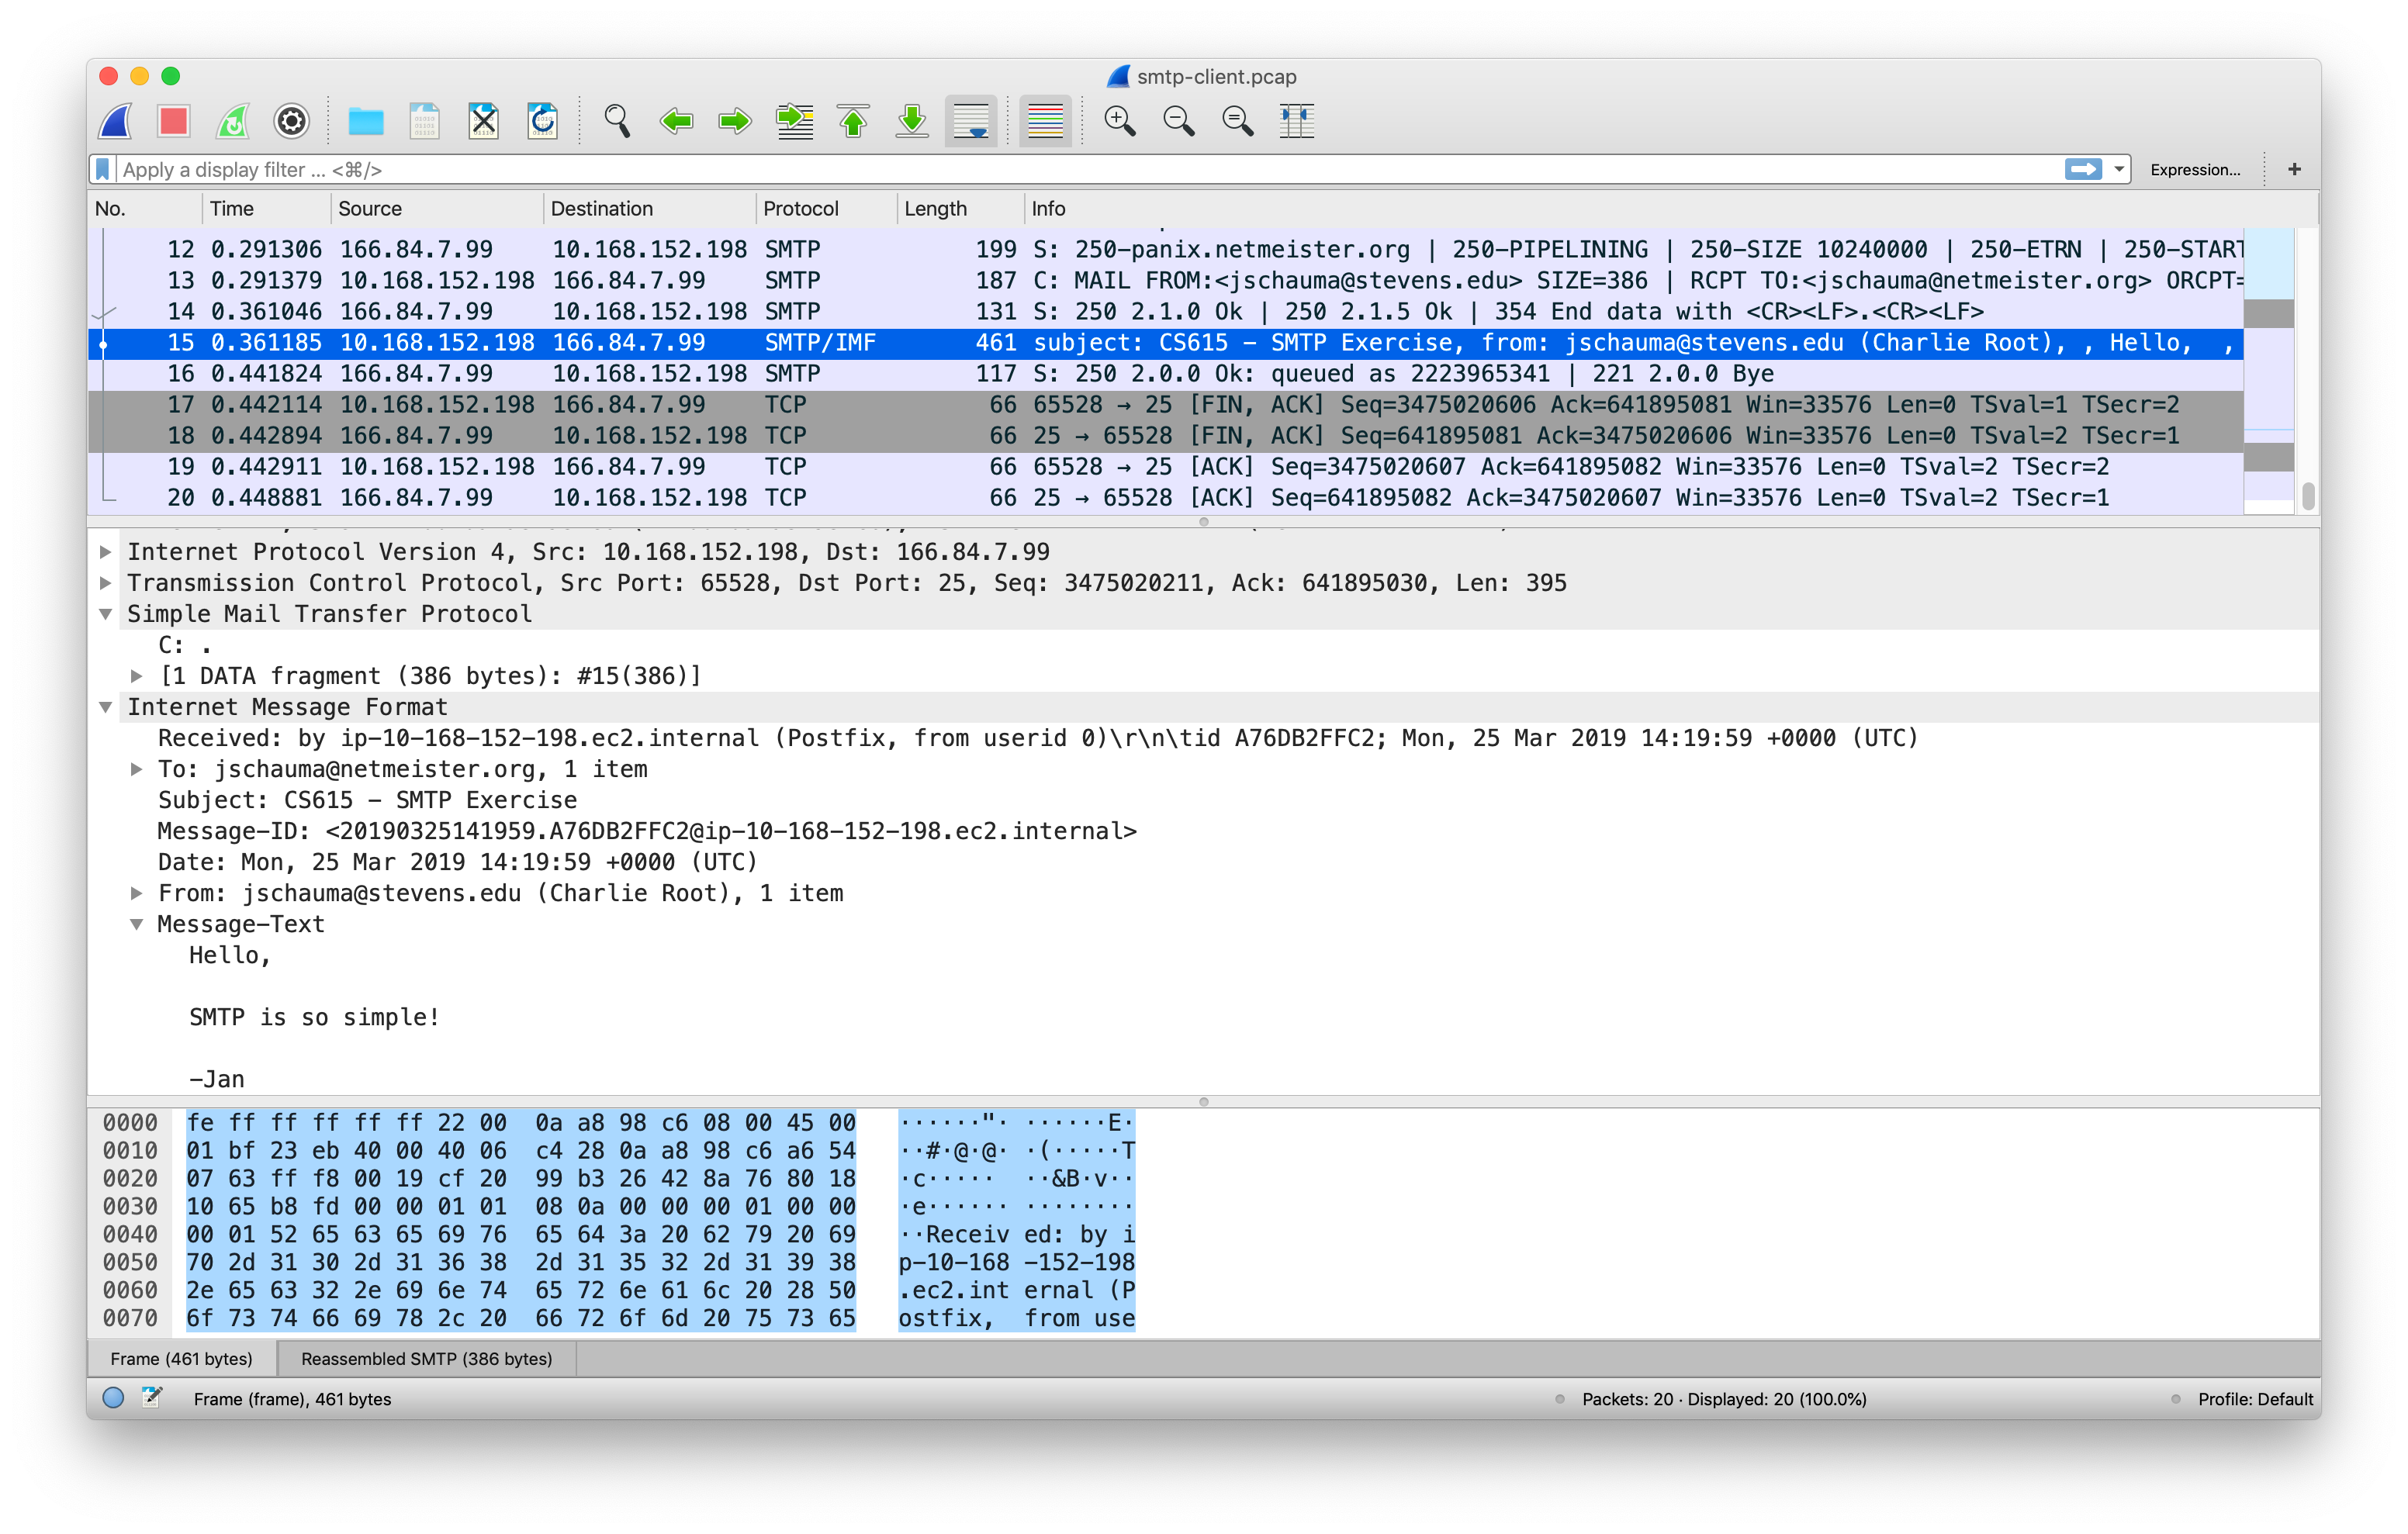
\includegraphics[scale=0.35]{pics/wireshark-smtp.eps}
%\end{center}
%
%\subsection{Sending...}
%\begin{Verbatim}
%$ telnet stevens-edu.mail.protection.outlook.com 25
%Trying 104.47.38.36...
%Connected to stevens-edu.mail.protection.outlook.com.
%Escape character is '^]'.
%220 BL2NAM02FT006.mail.protection.outlook.com Microsoft ESMTP MAIL Service
%    ready at Mon, 25 Mar 2019 02:06:53 +0000
%\textbf{EHLO ip-10-168-152-198.ec2.internal}
%250-BL2NAM02FT006.mail.protection.outlook.com Hello [54.160.173.145]
%[...]
%\textbf{MAIL FROM: <jschauma@stevens.edu>}
%250 2.1.0 Sender OK
%\textbf{RCPT TO: <jschauma@stevens.edu>}
%250 2.1.5 Recipient OK
%\end{Verbatim}
%
%\subsection{Sending...}
%\begin{Verbatim}
%\textbf{DATA}
%354 Start mail input; end with <CRLF>.<CRLF>
%\textbf{To: jschauma@stevens.edu}
%\textbf{Subject: CS615 - SMTP Exercise}
%\textbf{Date: Sat, 23 Mar 2019 20:52:04 +0000}
%\textbf{From: Charlie Root jschauma@stevens.edu}
%
%\textbf{Hello,}
%
%\textbf{SMTP is so simple!}
%
%\textbf{-Jan}
%\textbf{.}
%250 2.6.0 <<20190323205204.A89022FFB4@ip-10-183-182-79.ec2.internal>
%             > [InternalId=3397319131349,
%             > Hostname=BN6PR10MB1730.namprd10.prod.outlook.com]
%             7625 bytes in 9.276, 0.803 KB/sec Queued mail for delivery
%\end{Verbatim}
%
%\subsection{Receiving...}
%\small
%\begin{verbatim}
%IP 166.84.7.99.25 > 104.47.34.59.26730: Flags [P.], seq 1:41, ack 1,
%        SMTP: 220 panix.netmeister.org ESMTP Postfix
%IP 104.47.34.59.26730 > 166.84.7.99.25: Flags [P.], seq 1:53, ack 41,
%        SMTP: EHLO NAM01-BY2-obe.outbound.protection.outlook.com
%IP 166.84.7.99.25 > 104.47.34.59.26730: Flags [P.], seq 41:174, ack 53,
%        SMTP: 250-panix.netmeister.org
%IP 104.47.34.59.26730 > 166.84.7.99.25: Flags [P.], seq 53:63, ack 174,
%        STARTTLS
%IP 166.84.7.99.25 > 104.47.34.59.26730: Flags [P.], seq 174:204,
%        SMTP: 220 2.0.0 Ready to start TLS
%IP 104.47.34.59.26730 > 166.84.7.99.25: Flags [P.], seq 63:184, ack 204, SMTP
%IP 166.84.7.99.25 > 104.47.34.59.26730: Flags [.], seq 204:1664, ack 184, SMTP
%IP 166.84.7.99.25 > 104.47.34.59.26730: Flags [.], seq 1664:3124, ack 184, SMTP
%IP 104.47.34.59.26730 > 166.84.7.99.25: Flags [.], ack 3124, win 256, length 0
%IP 166.84.7.99.25 > 104.47.34.59.26730: Flags [P.], seq 3124:3720, ack 184, SMTP
%IP 104.47.34.59.26730 > 166.84.7.99.25: Flags [P.], seq 184:366, ack 3720, SMTP
%IP 166.84.7.99.25 > 104.47.34.59.26730: Flags [P.], seq 3720:4002, ack 366, SMTP
%IP 104.47.34.59.26730 > 166.84.7.99.25: Flags [P.], seq 366:499, ack 4002, SMTP
%IP 166.84.7.99.25 > 104.47.34.59.26730: Flags [P.], seq 4002:4215, ack 499, SMTP
%IP 104.47.34.59.26730 > 166.84.7.99.25: Flags [.], ack 4215, win 252, length 0
%IP 104.47.34.59.26730 > 166.84.7.99.25: Flags [P.], seq 499:664, ack 4215, SMTP
%\end{verbatim}
%\Normalsize
%
%\subsection{Receiving...}
%\begin{center}
%	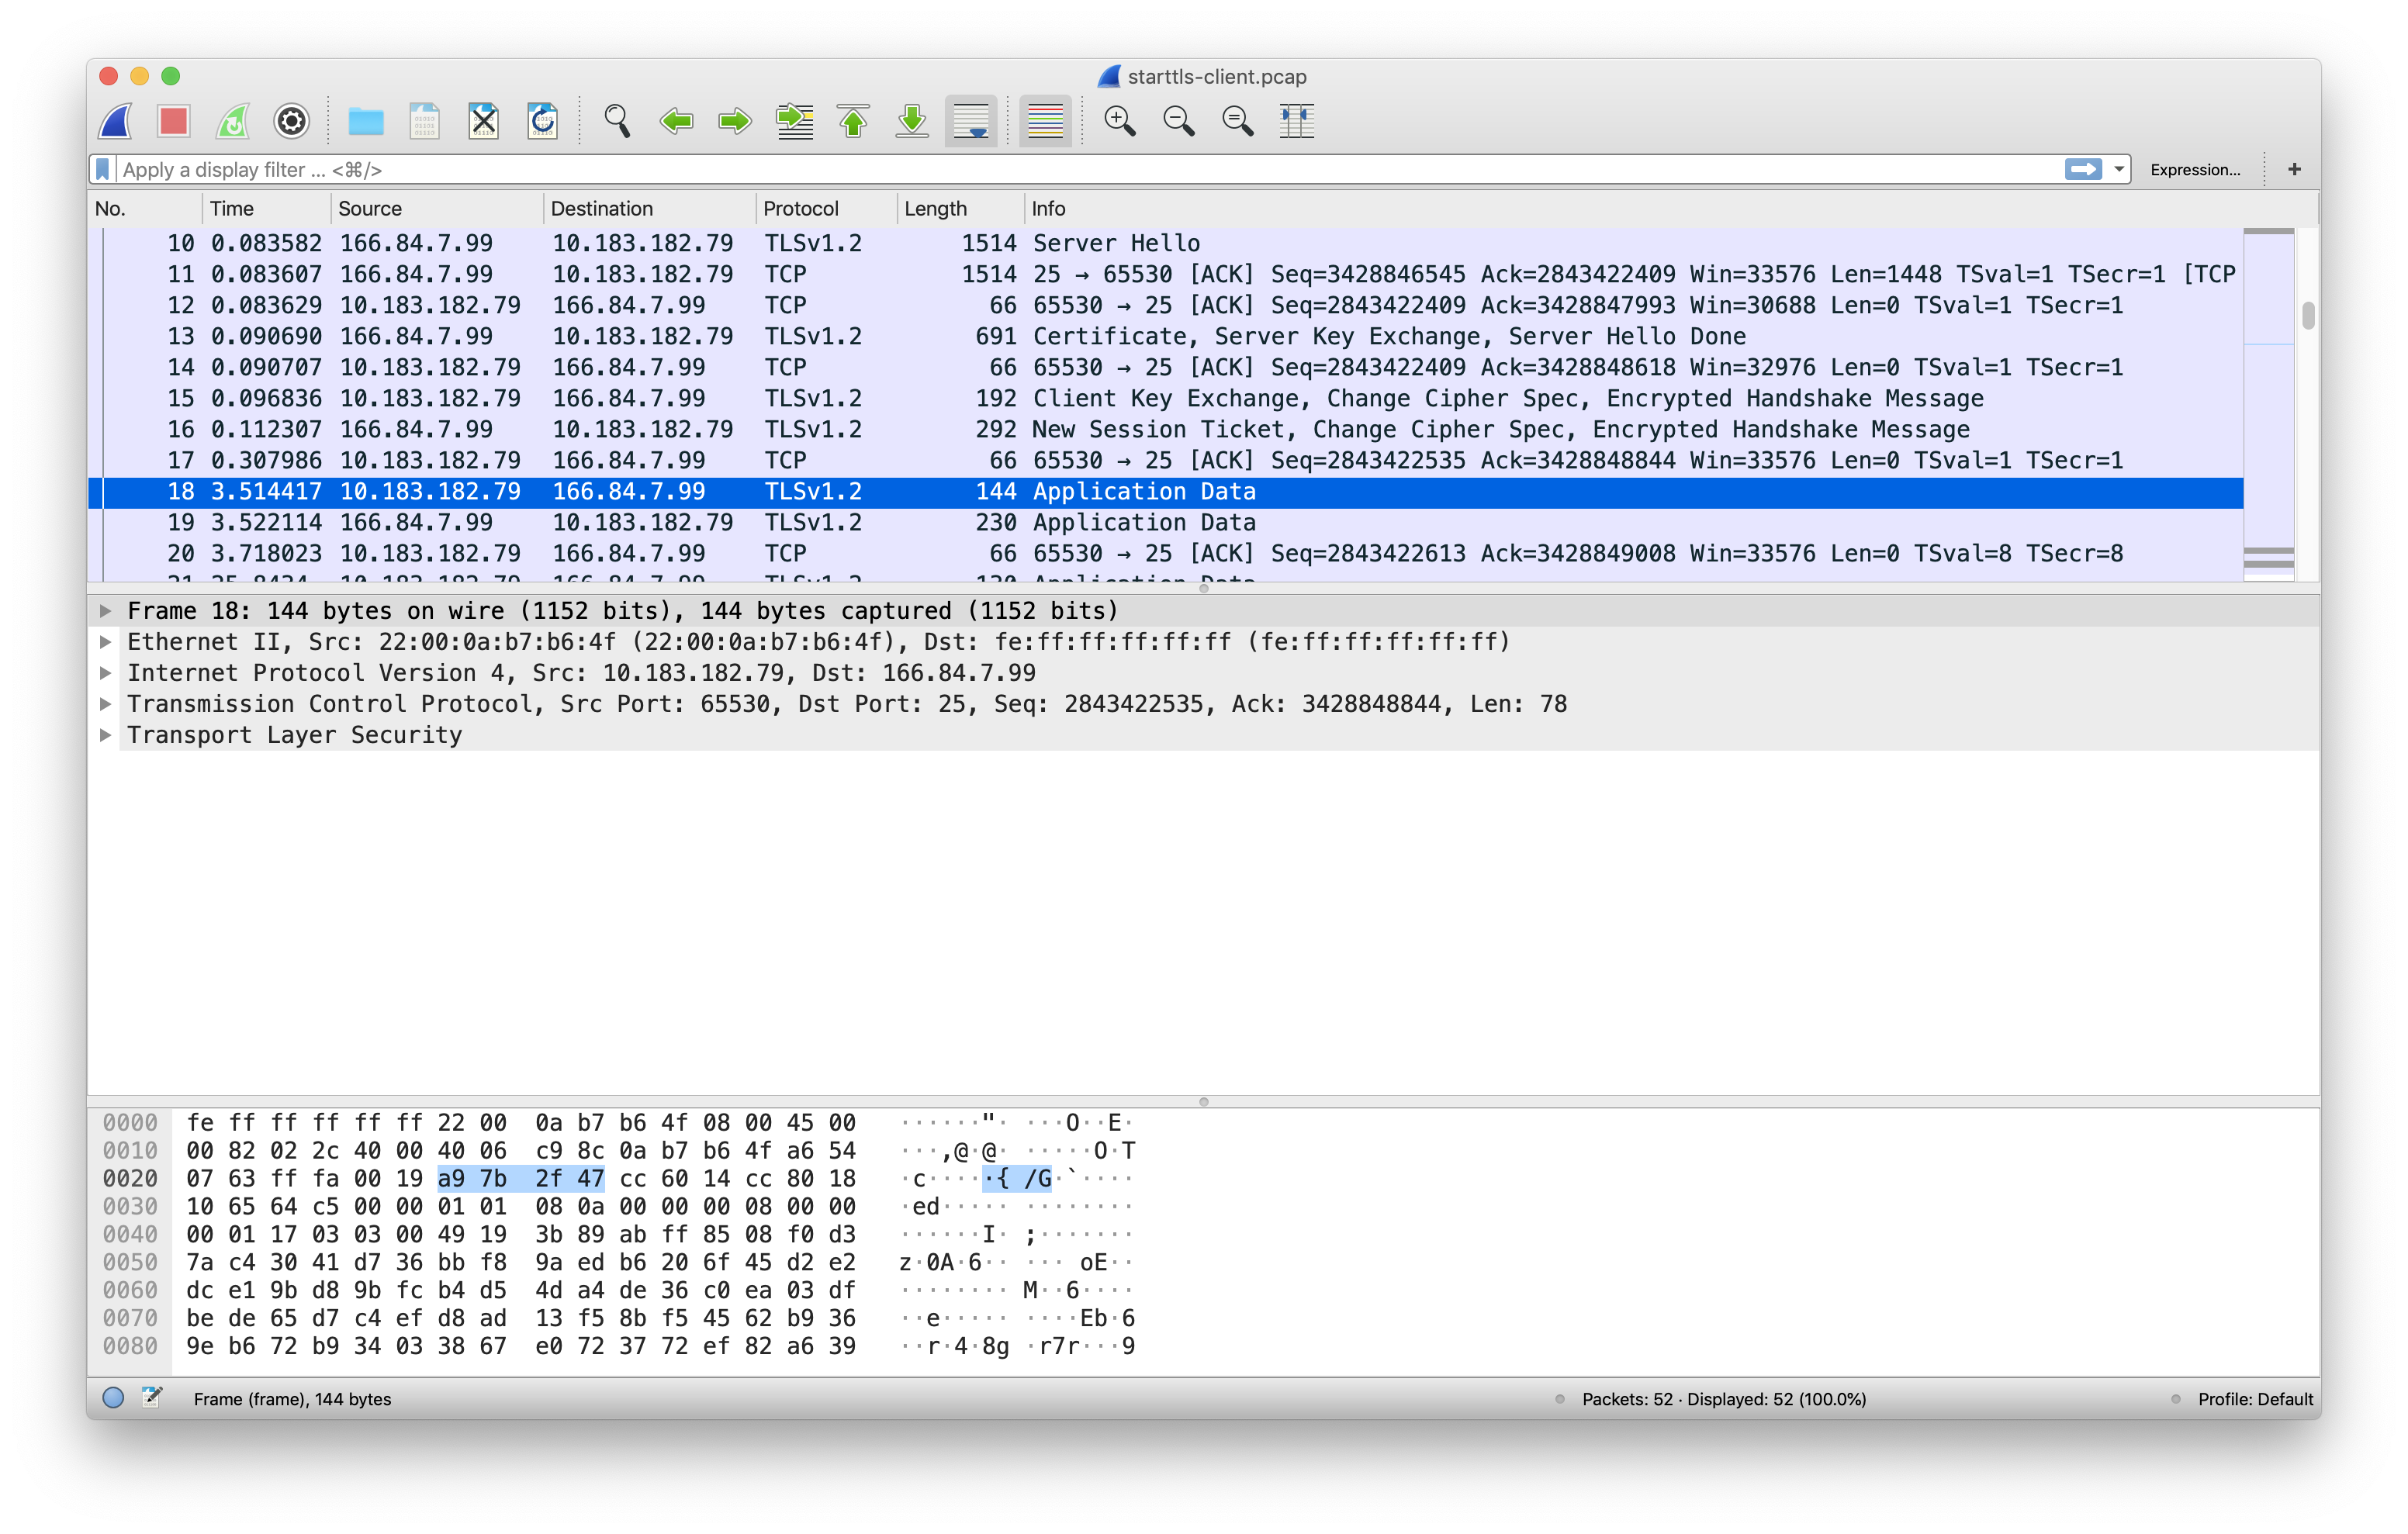
\includegraphics[scale=0.35]{pics/wireshark-smtp-tls.eps}
%\end{center}
%
%
%\subsection{Receiving...}
%\smallish
%\begin{verbatim}
%$ tail -f /var/log/maillog
%postfix/smtpd[7933]: connect from nexus.stevens.edu[155.246.14.12]
%postfix/smtpd[7933]: Anonymous TLS connection established from
%        nexus.stevens.edu[155.246.14.12]: TLSv1.2 with cipher AECDH-AES256-SHA (256/256 bits)
%postfix/smtpd[7933]: 6D2A1650D8: client=nexus.stevens.edu[155.246.14.12]
%postfix/cleanup[19825]: 6D2A1650D8: message-id=<943d7213a0a54930a35db5c0b0e94de2@exchng03.campus.stevens-tech.edu>
%postfix/cleanup[19825]: 6D2A1650D8: resent-message-id=<20180317192418.1B4111814A1@nexus.stevens.edu>
%postfix/qmgr[1885]: 6D2A1650D8: from=<jschauma@stevens.edu>, size=3456, nrcpt=1 (queue active)
%postfix/smtpd[7933]: disconnect from nexus.stevens.edu[155.246.14.12]
%postfix/pickup[9347]: DA65C65140: uid=1004 from=<jschauma@stevens.edu>
%postfix/cleanup[19825]: DA65C65140: message-id=<943d7213a0a54930a35db5c0b0e94de2@exchng03.campus.stevens-tech.edu>
%postfix/cleanup[19825]: DA65C65140: resent-message-id=<20180317192418.1B4111814A1@nexus.stevens.edu>
%postfix/qmgr[1885]: DA65C65140: from=<jschauma@stevens.edu>, size=3803, nrcpt=1 (queue active)
%postfix/local[9885]: DA65C65140: to=<jschauma@netmeister.org>, relay=local,
%        delay=0.22, delays=0.09/0/0/0.13, dsn=2.0.0,
%        status=sent (delivered to command: /usr/pkg/bin/procmail)
%postfix/qmgr[1885]: DA65C65140: removed
%\end{verbatim}
%\Normalsize
%

\subsection{Receiving...}
\begin{verbatim}
Date: Mon, 25 Mar 2019 14:19:59 +0000 (UTC)                                                         
From: Charlie Root <jschauma@stevens.edu>                                                           
To: jschauma@netmeister.org                                                                         
Subject: CS615 - SMTP Exercise                                                                      

Hello,

SMTP is so simple!

-Jan
\end{verbatim}

\subsection{STARTSSL}
\begin{verbatim}
EHLO ec2-54-160-173-145.compute-1.amazonaws.com
250-panix.netmeister.org
250-PIPELINING
250-SIZE 10240000
250-ETRN
250-STARTTLS
250-ENHANCEDSTATUSCODES
250-8BITMIME
250 DSN
STARTTLS
220 2.0.0 Ready to start TLS
now what?
Connection closed by foreign host.
\end{verbatim}

\subsection{STARTSSL}
\begin{verbatim}
$ openssl s_client -starttls smtp -crlf -connect panix.netmeister.org:25
New, TLSv1/SSLv3, Cipher is ECDHE-RSA-AES256-GCM-SHA384
Server public key is 4096 bit
SSL-Session:
    Protocol  : TLSv1.2
    Cipher    : ECDHE-RSA-AES256-GCM-SHA384
[...]
helo ec2-54-160-173-145.compute-1.amazonaws.com
[...]
\end{verbatim}

\subsection{STARTTLS}
\begin{center}
	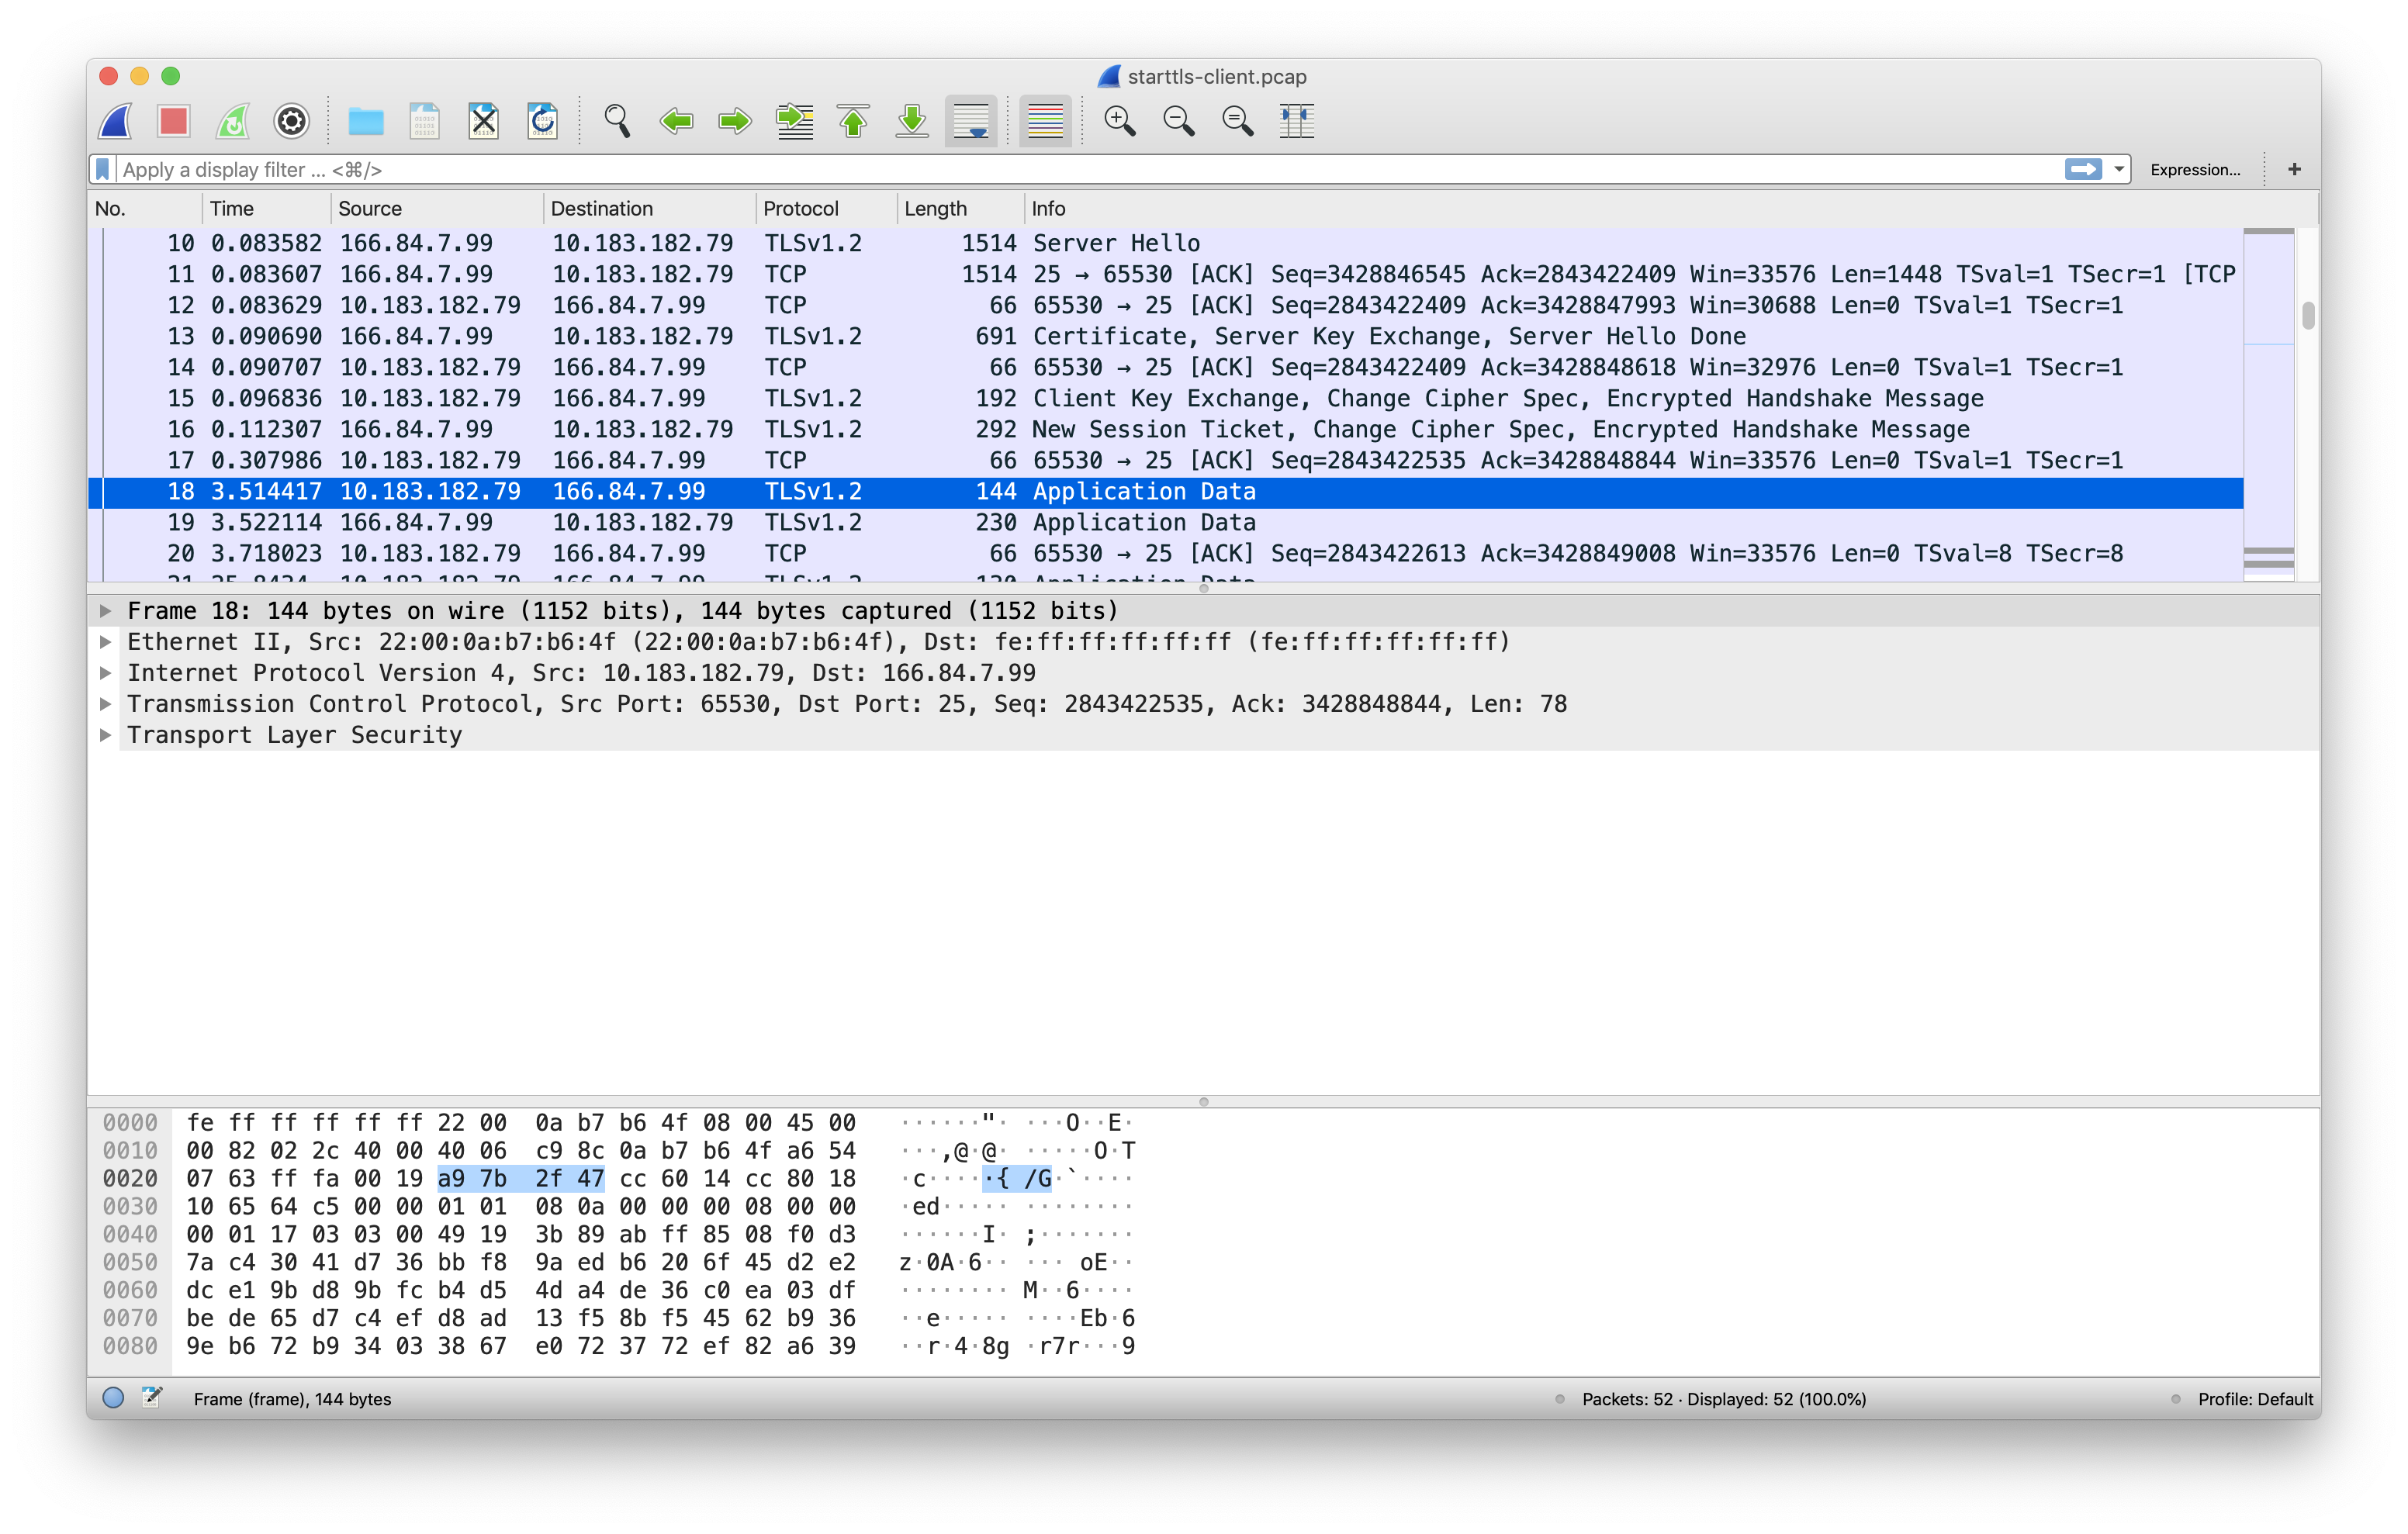
\includegraphics[scale=0.35]{pics/wireshark-smtp-tls.eps}
\end{center}

\subsection{STARTTLS is Opportunistic Encryption}
\begin{itemize}
	\item MitM can strip \verb+STARTTLS+
	\item Should failure to verify certificate lead to mail to being delivered?
	\item DNS-Based Authentication of Named Entities (DANE) (RFC7672)
	\item SMTP MTA Strict Transport Security (MTA-STS) (RFC8461)
\end{itemize}

\begin{verbatim}
$ host -t txt _mta-sts.yahoo.com
_mta-sts.yahoo.com descriptive text "v=STSv1; id=20161109010200Z;"
$ host -t txt _mta-sts.gmail.com
_mta-sts.gmail.com descriptive text "v=STSv1; id=20171114T070707;"
$ host -t txt _mta-sts.stevens.edu
Host _mta-sts.stevens.edu not found: 3(NXDOMAIN)
$ curl https://mta-sts.yahoo.com/.well-known/mta-sts.txt
version: STSv1
mode: testing
mx: *.am0.yahoodns.net
mx: *.mail.gm0.yahoodns.net
mx: *.mail.am0.yahoodns.net
max_age: 86400
\end{verbatim}

\subsection{Receiving...}
\begin{verbatim}
Date: Mon, 25 Mar 2019 14:19:59 +0000 (UTC)                                                         
From: Charlie Root <jschauma@stevens.edu>                                                           
To: jschauma@netmeister.org                                                                         
Subject: CS615 - SMTP Exercise                                                                      

Hello,

SMTP is so simple!

-Jan
\end{verbatim}

\subsection{Anatomy of an email message}
An email consists of:
\begin{itemize}
	\item mandatory headers (such as "From ", "Delivered-To: ", ...)
	\item optional headers (such as "From: ", "To: ", "Subject: ", ...)
	\item the body of the message
	\begin{itemize}
		\item content independent of SMTP
		\item Multipurpose Internet Mail Extensions (MIME) enables non-ascii, multipart, encodings, ...
	\end{itemize}
\end{itemize}


\subsection{Receiving...}
\smallish
\begin{verbatim}
From jschauma@stevens.edu  Mon Mar 25 10:20:21 2019
Return-Path: <jschauma@stevens.edu>
X-Original-To: jschauma@netmeister.org
Delivered-To: jschauma@netmeister.org
Received: by panix.netmeister.org (Postfix, from userid 1004)
        id 0E9C0654CE; Mon, 25 Mar 2019 10:20:21 -0400 (EDT)
X-Spam-Checker-Version: SpamAssassin 3.4.2 (2018-09-13) on panix.netmeister.org
X-Spam-Level: 
X-Spam-Status: No, score=0.5 required=5.0 tests=BAYES_05,RDNS_DYNAMIC
        autolearn=no autolearn_force=no version=3.4.2
Received: from ip-10-168-152-198.ec2.internal (ec2-54-160-173-145.compute-1.amazonaws.com [54.160.173.145])
        by panix.netmeister.org (Postfix) with ESMTP id 2223965341
        for <jschauma@netmeister.org>; Mon, 25 Mar 2019 10:20:01 -0400 (EDT)
Received: by ip-10-168-152-198.ec2.internal (Postfix, from userid 0)
        id A76DB2FFC2; Mon, 25 Mar 2019 14:19:59 +0000 (UTC)
To: jschauma@netmeister.org
Subject: CS615 - SMTP Exercise
Message-Id: <20190325141959.A76DB2FFC2@ip-10-168-152-198.ec2.internal>
Date: Mon, 25 Mar 2019 14:19:59 +0000 (UTC)
From: jschauma@stevens.edu (Charlie Root)
Status: RO
Content-Length: 33
Lines: 5
\end{verbatim}
\Normalsize

\subsection{Authenticity and SPAM}
\vspace*{\fill}
\begin{center}
	\includegraphics[scale=1.5]{pics/spam.eps} \\
	{\tt https://youtu.be/9OVKXIfrGJE}
\end{center}
\vspace*{\fill}

\subsection{Relaying mail}
\begin{verbatim}
$ telnet stevens-edu.mail.protection.outlook.com 25
Trying 104.47.36.36...
Connected to stevens-edu.mail.protection.outlook.com.
Escape character is '^]'.
220 SN1NAM02FT062.mail.protection.outlook.com Microsoft ESMTP MAIL Service
        ready at Mon, 25 Mar 2019 16:27:13 +0000
EHLO localhost
250 SN1NAM02FT062.mail.protection.outlook.com Hello [54.160.173.145]
MAIL FROM: <leaks@whitehouse.gov>
250 2.1.0 Sender OK
RCPT TO: <mueller@fbi.gov>
451 4.4.62 Mail sent to the wrong Office 365 region. ATTR35.
        For more information please go to https://go.microsoft.com/fwlink/?linkid=865268
        [SN1NAM02FT062.eop-nam02.prod.protection.outlook.com]
quit
221 2.0.0 Service closing transmission channel
Connection closed by foreign host.
\end{verbatim}

\subsection{Authenticity and SPAM}
\smallish
\begin{Verbatim}
220 panix.netmeister.org ESMTP Postfix
EHLO ec2-54-160-173-145.compute-1.amazonaws.com
250 panix.netmeister.org
MAIL FROM: <barack@obama.org>
250 2.1.0 Ok
\textbf{RCPT TO: <jschauma@netmeister.org>}
250 2.1.5 Ok
DATA
354 End data with <CR><LF>.<CR><LF>
From: "Barack Obama" <barack@obama.org>
\textbf{To: "Jan Schaumann" <jschauma@stevens.edu>}
Subject: Friday

Yo,

Party at my house.
BYOB.

-B
.
250 2.0.0 Ok: queued as \textbf{A1D5D65341}
\end{Verbatim}
\Normalsize

\subsection{Authenticity}
\begin{verbatim}
Date: Mon, 25 Mar 2019 13:09:06 -0400 (EDT)                                                         
From: Barack Obama <barack@obama.org>
To: Jan Schaumann <jschauma@stevens.edu>
Subject: Friday

Yo,

Party at my house.
BYOB.

-B
\end{verbatim}

\subsection{Receiving...}
\smallish
\begin{verbatim}
$ tail -f /var/log/maillog
<mail.info>Mar 25 13:08:31 panix postfix/smtpd[15759]:
        connect from ec2-54-160-173-145.compute-1.amazonaws.com[54.160.173.145] 
<mail.info>Mar 25 13:08:38 panix postfix/smtpd[15759]: A1D5D65341:
        client=ec2-54-160-173-145.compute-1.amazonaws.com[54.160.173.145]
<mail.info>Mar 25 13:08:46 panix postfix/cleanup[15274]: A1D5D65341:
        message-id=<>
<mail.info>Mar 25 13:08:46 panix postfix/qmgr[1932]: A1D5D65341:
        from=<barack@obama.org>, size=396, nrcpt=1 (queue active)
<mail.info>Mar 25 13:08:46 panix spamd[18739]: spamd:
        clean message (4.8/5.0) for spamd:1004 in 0.2 seconds, 383 bytes.
<mail.info>Mar 25 13:08:46 panix spamd[18739]: spamd:
        result: . 4 - BAYES_40,HELO_DYNAMIC_IPADDR,MISSING_DATE,MISSING_MID,RDNS_DYNAMIC
        scantime=0.2,size=383,user=spamd,uid=1004,required_score=5.0,
        rhost=::1,raddr=::1,rport=59084,mid=(unknown),bayes=0.258339,autolearn=no
        autolearn_force=no
<mail.info>Mar 25 13:08:48 panix postfix/smtpd[15759]:
        disconnect from ec2-54-160-173-145.compute-1.amazonaws.com[54.160.173.145]
<mail.info>Mar 25 13:09:06 panix postfix/qmgr[1932]: A1D5D65341: removed
\end{verbatim}
\Normalsize

\subsection{Authenticity and SPAM}
\smallish
\begin{verbatim}
$ tcpdump -n -t -r smtp-spam-server.pcap port 53
IP 166.84.7.99.60228 > 166.84.67.2.53: 10483+ PTR? 145.173.160.54.in-addr.arpa. (45)
IP 166.84.67.2.53 > 166.84.7.99.60228: 10483 1/5/6 PTR ec2-54-160-173-145.compute-1.amazonaws.com. (322)
IP 166.84.7.99.60227 > 166.84.67.2.53: 8466+ A? ec2-54-160-173-145.compute-1.amazonaws.com. (60)
IP 166.84.67.2.53 > 166.84.7.99.60227: 8466 1/13/9 A 54.160.173.145 (502)
IP 166.84.7.99.60226 > 166.84.67.2.53: 23794+ MX? obama.org. (27)
IP 166.84.67.2.53 > 166.84.7.99.60226: 23794 5/2/12 MX aspmx.l.google.com. 1,
        MX aspmx3.googlemail.com. 10, MX aspmx2.googlemail.com. 10,
        MX alt2.aspmx.l.google.com. 5, MX alt1.aspmx.l.google.com. 5 (501)
IP 166.84.7.99.60225 > 166.84.67.2.53: 22084+ A? ec2-54-160-173-145.compute-1.amazonaws.com. (60)
IP 166.84.67.2.53 > 166.84.7.99.60225: 22084 1/13/9 A 54.160.173.145 (502)
IP 166.84.7.99.60224 > 166.84.67.2.53: 13128+ A? 145.173.160.54.sbl.spamhaus.org. (49)
IP 166.84.67.2.53 > 166.84.7.99.60224: 13128 NXDomain 0/1/0 (113)
IP 166.84.7.99.56261 > 166.84.67.2.53: 40648+ [1au] A? 145.173.160.54.bl.mailspike.net. (60)
IP 166.84.7.99.56261 > 166.84.67.2.53: 15871+ [1au] A? 145.173.160.54.dnsbl.sorbs.net. (59)
IP 166.84.7.99.56261 > 166.84.67.2.53: 62257+ [1au] TXT? 145.173.160.54.sa-accredit.habeas.com. (66)
IP 166.84.7.99.56261 > 166.84.67.2.53: 6046+ [1au] A? 145.173.160.54.wl.mailspike.net. (60)
IP 166.84.7.99.56261 > 166.84.67.2.53: 59439+ [1au] A? 145.173.160.54.iadb.isipp.com. (58)
IP 166.84.67.2.53 > 166.84.7.99.56261: 15871 NXDomain 0/1/1 (115)
IP 166.84.7.99.56261 > 166.84.67.2.53: 21500+ [1au] A? 145.173.160.54.bl.score.senderscore.com. (68)
IP 166.84.7.99.56261 > 166.84.67.2.53: 4312+ [1au] A? 145.173.160.54.zen.spamhaus.org. (60)
IP 166.84.67.2.53 > 166.84.7.99.56261: 59439 NXDomain 0/1/1 (105)
IP 166.84.67.2.53 > 166.84.7.99.56261: 21500 NXDomain 0/1/1 (130)
IP 166.84.7.99.56261 > 166.84.67.2.53: 33947+ [1au] TXT? 145.173.160.54.sa-trusted.bondedsender.org. (71)
IP 166.84.7.99.56261 > 166.84.67.2.53: 33325+ [1au] A? 145.173.160.54.list.dnswl.org. (58)
IP 166.84.7.99.56261 > 166.84.67.2.53: 60189+ [1au] TXT? 145.173.160.54.bl.spamcop.net. (58)
IP 166.84.67.2.53 > 166.84.7.99.56261: 33325 NXDomain 0/1/1 (106)
IP 166.84.7.99.56261 > 166.84.67.2.53: 63286+ [1au] A? 145.173.160.54.psbl.surriel.com. (60)
IP 166.84.67.2.53 > 166.84.7.99.56261: 63286 NXDomain 0/1/1 (109)
IP 166.84.67.2.53 > 166.84.7.99.56261: 4312 NXDomain 0/1/1 (124)
IP 166.84.67.2.53 > 166.84.7.99.56261: 62257 NXDomain 0/0/1 (66)
IP 166.84.67.2.53 > 166.84.7.99.56261: 33947 NXDomain 0/0/1 (71)
IP 166.84.67.2.53 > 166.84.7.99.56261: 60189 NXDomain 0/1/1 (111)
IP 166.84.7.99.56261 > 166.84.67.2.53: 8981+ [1au] TXT? _adsp._domainkey.obama.org. (55)
IP 166.84.67.2.53 > 166.84.7.99.56261: 8981 0/1/1 (117)
IP 166.84.7.99.56261 > 166.84.67.2.53: 19917+ [1au] MX? obama.org. (38)
IP 166.84.67.2.53 > 166.84.7.99.56261: 19917 5/2/14 MX alt2.aspmx.l.google.com. 5, MX aspmx2.googlemail.com. 10, MX alt1.aspmx.l.google.com. 5, MX aspmx.l.google.com. 1, MX aspmx3.googlemail.com. 10 (540)
IP 166.84.7.99.56261 > 166.84.67.2.53: 35638+ [1au] TXT? ec2-54-160-173-145.compute-1.amazonaws.com. (71)
IP 166.84.67.2.53 > 166.84.7.99.56261: 35638 0/1/1 (139)
IP 166.84.67.2.53 > 166.84.7.99.56261: 40648 NXDomain 0/0/1 (60)
IP 166.84.67.2.53 > 166.84.7.99.56261: 6046 NXDomain 0/0/1 (60)
\end{verbatim}
\Normalsize

\subsection{Authenticity and SPAM}
\smallish
\begin{verbatim}
IP 166.84.7.99.25 > 155.246.14.12.49256: Flags [F.], seq 1064, ack 4009
IP 166.84.7.99.42727 > 166.84.67.2.53: 36601 [1au] A? 12.14.246.155.zen.spamhaus.org. (59)
IP 166.84.7.99.42727 > 166.84.67.2.53: 64419 [1au] TXT? 12.14.246.155.sa-trusted.bondedsender.org. (70)
IP 166.84.7.99.42727 > 166.84.67.2.53: 5389 [1au] A? 12.14.246.155.psbl.surriel.com. (59)
IP 166.84.67.2.53 > 166.84.7.99.42727: 36601 0/20/141 (1472)
IP 166.84.7.99.42727 > 166.84.67.2.53: 46848 [1au] A? 12.14.246.155.bb.barracudacentral.org. (66)
IP 166.84.67.2.53 > 166.84.7.99.42727: 64419 0/18/19 (1148)
IP 166.84.67.2.53 > 166.84.7.99.42727: 5389 0/4/6 (266)
IP 166.84.67.2.53 > 166.84.7.99.42727: 46848 0/3/7 (264)
IP 166.84.7.99.42727 > 166.84.67.2.53: 60194 [1au] A? 12.14.246.155.bl.mailspike.net. (59)
IP 166.84.67.2.53 > 166.84.7.99.42727: 60194 0/3/4 (183)
IP 166.84.7.99.42727 > 166.84.67.2.53: 17555 [1au] A? 36.248.246.155.zen.spamhaus.org. (60)
IP 166.84.7.99.42727 > 166.84.67.2.53: 12591 [1au] A? 6.2.8.f.6.f.b.9.0.0.0.0.0.0.0.0.0.0.0.0.6.2.8.f.6.f.b.9.2.0.0.2.zen.spamhaus.org. (109)
IP 166.84.7.99.42727 > 166.84.67.2.53: 3616 [1au] A? 21.14.246.155.zen.spamhaus.org. (59)
IP 166.84.67.2.53 > 166.84.7.99.42727: 17555 0/20/141 (1472)
IP 166.84.7.99.42727 > 166.84.67.2.53: 22783 [1au] A? 12.14.246.155.bl.score.senderscore.com. (67)
IP 166.84.67.2.53 > 166.84.7.99.42727: 12591 0/20/141 (1472)
IP 166.84.7.99.42727 > 166.84.67.2.53: 48053 [1au] A? 12.14.246.155.list.dnswl.org. (57)
IP 166.84.67.2.53 > 166.84.7.99.42727: 3616 0/20/141 (1472)
IP 166.84.67.2.53 > 166.84.7.99.42727: 22783 NXDomain 0/1/1 (129)
IP 166.84.67.2.53 > 166.84.7.99.42727: 48053 1/5/13 A 127.0.11.2 (420)
IP 166.84.7.99.42727 > 166.84.67.2.53: 25189 [1au] TXT? 36.248.246.155.bl.spamcop.net. (58)
IP 166.84.67.2.53 > 166.84.7.99.42727: 25189 0/8/9 (422)
IP 166.84.7.99.42727 > 166.84.67.2.53: 25751 [1au] TXT? 21.14.246.155.bl.spamcop.net. (57)
\end{verbatim}
\Normalsize

\subsection{Sender Policy Framework}
{\em SPF} (RFC7208) can help detect email spoofing by identifying the
list of allowed sending MXs by way of specifically
formatted {\tt TXT} records. \\

\begin{verbatim}
$ host -t txt obama.org | grep spf
obama.org descriptive text "v=spf1 include:_spf.salesforce.com include:_spf.google.com
        include:bounce.bluestatedigital.com include:sendgrid.net ~all"
$ host -t txt yahoo.com | grep spf
yahoo.com descriptive text "v=spf1 redirect=_spf.mail.yahoo.com"
$ host -t txt _spf.mail.yahoo.com | grep spf
_spf.mail.yahoo.com descriptive text "v=spf1 ptr:yahoo.com ptr:yahoo.net ?all"
$ host -t txt netmeister.org | grep spf
netmeister.org descriptive text "v=spf1 a mx ~all"
$ 
\end{verbatim}

\subsection{Sender Policy Framework}
Softfail:
\begin{verbatim}
$ host -t txt obama.org | grep spf
obama.org descriptive text "v=spf1 include:_spf.salesforce.com include:_spf.google.com
        include:bounce.bluestatedigital.com include:sendgrid.net ~all"


Authentication-Results: spf=softfail (sender IP is 54.160.173.145)
        smtp.mailfrom=obama.org; stevens.edu; dkim=none (message not signed)
        header.d=none;stevens.edu; dmarc=fail action=oreject
        header.from=obama.org;compauth=fail reason=000
Received-SPF: SoftFail (protection.outlook.com: domain of transitioning
        obama.org discourages use of 54.160.173.145 as permitted sender)
\end{verbatim}

\subsection{Sender Policy Framework}
Hardfail:
\begin{verbatim}
$ host -t txt stevens.edu | grep spf
stevens.edu descriptive text "v=spf1 ip4:155.246.0.0/16 include:_netblocks.google.com
        include:_netblocks2.google.com include:spf.protection.outlook.com include:_spf.acquia.com ip4:216.235.196.0/22 ip4:216.235.200.0/21 ip4:205.139.104.0/22
        ip4:52.35.7.203 ip4:74.208.4.192/26 " " ip4:66.132.220.97 ip4:198.187.196.100 ip4:66.45.4.80
        ip4:66.132.220.95 -all"

Authentication-Results: spf=fail (sender IP is 54.160.173.145)
        smtp.mailfrom=stevens.edu; stevens.edu; dkim=none (message not signed)
        header.d=none;stevens.edu; dmarc=none action=none
        header.from=stevens.edu;compauth=fail reason=601
Received-SPF: Fail (protection.outlook.com: domain of stevens.edu does not
        designate 54.160.173.145 as permitted sender)
        receiver=protection.outlook.com; client-ip=54.160.173.145;
        helo=ip-10-168-152-198.ec2.internal;
\end{verbatim}

\subsection{DomainKeys Identified Mail aka {\tt DKIM}}
{\em DKIM} can help detect email spoofing by providing a
digital signature across parts of the message.

\begin{itemize}
	\item developed by Yahoo with help from Cisco, PGP, and Sendmail
	\item RFC4871, published in 2007, updated via RFC6376
	\item {\tt DKIM-Signature} headers
	\item more DNS {\tt TXT} records (\verb+<s>._domainkey.<d>+) -- we really rely on and trust DNS quite a bit, don't we?
\end{itemize}

\subsection{DKIM Example}
\begin{verbatim}
DKIM-Signature: v=1; a=rsa-sha256; c=relaxed/relaxed;                                               
        d=stevens0.onmicrosoft.com; s=selector1-stevens-edu;                                        
        h=From:Date:Subject:Message-ID:Content-Type:
        MIME-Version:X-MS-Exchange-SenderADCheck;       
        bh=JACUpIBf890+LLb3naV0x1KcKzH82I+/G5T/iFkDj2A=;                                            
        b=Qa4evi5FIY6z+5i8B70m0wxLIFwh5cVPRLFxhoorepLJ1q5/LfKdouIam6+MXhXj1u1EDmG
        jzeVDXu45xjrgkqctUrjE/Ykz5/6mEGLeVb8s4t56FNGKPKiz3UCZ4+ojqHt8tMwOpn8o675Kwa68nCISUP9I740jd0V6eLRNGSQ=                  

$ host -t txt selector1-stevens-edu._domainkey.stevens0.onmicrosoft.com
selector1-stevens-edu._domainkey.stevens0.onmicrosoft.com
descriptive text "v=DKIM1; k=rsa; p=MIGfMA0GCSqGSIb3DQEBAQUAA4GNADCBiQKBgQCk/
JSw4q2rARSBhh/vPn1mOmDpitEG2PsUz59tT0jt5R4QAsvKyaJAmtdnBQXtxZiVakZDTeIKY9gpZ4
lvL0o7FSNeUsxZHkQZoLkN+f6q6Zipdag9zIS+R0a9DC2AmIqKX6g14TkIxOprJgAvlD57nCGyX8L
io4pVfFLK6lCYTwIDAQAB; n=1024,1452130342,1"
\end{verbatim}
\vspace{.5in}

\subsection{Domain-based Message Authentication, Reporting and Conformance}
{\em DMARC} provides a policy of which validation
mechanisms should be employed for a given domain.

\begin{itemize}
	\item RFC7489
	\item uses SPF and DKIM
	\item more DNS {\tt TXT} records (\verb+_dmarc.<domain>+)
	\item extends across {\tt From} and {\tt From: } alignment
	\item provides report mechanism
\end{itemize}
\vspace{.25in}

\begin{verbatim}
$ dig +short txt _dmarc.yahoo.com
"v=DMARC1; p=reject; pct=100; rua=mailto:dmarc_y_rua@yahoo.com;"
\end{verbatim}

\subsection{DMARC in action}
\smallish
\begin{verbatim}
$  telnet gmail-smtp-in.l.google.com 25
Trying 172.217.197.27...
Connected to gmail-smtp-in.l.google.com.
Escape character is '^]'.
220 mx.google.com ESMTP q16si1000312qtb.313 - gsmtp
EHLO ec2-54-160-173-145.compute-1.amazonaws.com
250 mx.google.com at your service
MAIL FROM: <jschauma@yahoo.com>
250 2.1.0 OK q16si1000312qtb.313 - gsmtp
RCPT TO: <jschauma@gmail.com>
250 2.1.5 OK q16si1000312qtb.313 - gsmtp
DATA
354  Go ahead q16si1000312qtb.313 - gsmtp
Subject: DMARC fail
From: jschauma@yahoo.com

This should fail.
.
550-5.7.1 Unauthenticated email from yahoo.com is not accepted due to domain's
550-5.7.1 DMARC policy. Please contact the administrator of yahoo.com domain if
550-5.7.1 this was a legitimate mail. Please visit 550-5.7.1
          https://support.google.com/mail/answer/2451690 to learn about the
550 5.7.1 DMARC initiative. q16si1000312qtb.313 - gsmtp
\end{verbatim}
\Normalsize

\subsection{SMTP is a Simple Mail Transfer Protocol.}
\begin{itemize}
	\item TCP port 25
	\item DNS MX records
	\item mail may be relayed or processed by many servers in transit
	\item transport is in clear text
	\item STARTTLS may provide (opportunistic) transport encryption
	\item SPAM controls may include DNS lookups, bayesian scoring, ...
	\item authenticity not guaranteed, although DMARC, DKIM, SPF can help
\end{itemize}

\subsection{Service Considerations}
\begin{itemize}
	\item outsourcing versus in-house
	\item privacy considerations
	\item spam protections
	\item phishing protections
	\item mail delivery cannons for notifications vs. spam lists
	\item high volume traffic demands fine-tuned systems
	\item high volume traffic implications on logging
\end{itemize}
\vspace{.5in}
See also:
\begin{itemize}
	\item {\tt https://is.gd/JQp1zM}
	\item {\tt https://is.gd/cXyrwX}
	\item {\tt https://is.gd/o6Y5f8}
\end{itemize}

\subsection{Reading}
SMTP
\begin{itemize}
	\item SMTP: {\tt https://tools.ietf.org/html/rfc5321}
	\item Message format: {\tt https://tools.ietf.org/html/rfc5322}
	\item SPF: {\tt https://tools.ietf.org/html/rfc7208}
	\item DKIM: {\tt https://is.gd/VnCO9f}, {\tt https://tools.ietf.org/html/rfc6376}
	\item DMARC: {\tt https://tools.ietf.org/html/rfc7489}
	\item DANE: {\tt https://tools.ietf.org/html/rfc7672}
	\item MTA-STS: {\tt https://tools.ietf.org/html/rfc8461.html}
\end{itemize}

\subsection{Reading}
HTTPS / TLS:
\begin{itemize}
	\item {\tt https://en.wikipedia.org/wiki/HTTPS}
	\item RFC5246 (TLS 1.2) and RFC6176 (prohibiting SSL)
	\item RFC8446 (TLS 1.3)
	\item {\tt https://bugzilla.mozilla.org/show\_bug.cgi?id=647959}
	\item {\tt https://cabforum.org}
	\item {\tt https://jhalderm.com/pub/papers/interception-ndss17.pdf}
	\item {\tt https://tls.ulfheim.net/} / {\tt https://tls13.ulfheim.net/}
\end{itemize}

%http://websocketd.com/

\end{document}
